% !TEX root = ../../技术文档.tex
\section{CPU仿真验证}

\subsection{指令集验证}

本节指令集回归采用单发射\texttt{rv32im\_zicsr}配置；双发射的参数组合与关键接口检查列于系统级仿真验证。
回归用例分别取自\texttt{riscv-tests}\cite{riscv-tests}和基于ACT4框架的RISC-V架构测试集\cite{riscv-act4}。
\texttt{riscv-tests}功能测试结果为\textbf{50/50 PASS}，ACT4架构一致性测试结果为\textbf{53/53 PASS}。
支撑材料保存于\path{docs/verification/cpu/isa_support/}。

\subsubsection{riscv-tests逐项结果}
表\ref{tbl:cpu-riscv-tests-cases}列出RV32I的40项、RV32M的8项及机器CSR的2项测试。

\begin{reporttable}
\begin{longtable}{@{}r p{0.22\linewidth}p{0.12\linewidth}p{0.39\linewidth}p{0.13\linewidth}@{}}
\caption{riscv-tests逐项用例清单（50/50 PASS）}\label{tbl:cpu-riscv-tests-cases}\\
\toprule
序号 & 配置 & 指令集 & 用例 & 状态 \\
\midrule
\endfirsthead
\caption[]{riscv-tests逐项用例清单（50/50 PASS）（续）}\\
\toprule
序号 & 配置 & 指令集 & 用例 & 状态 \\
\midrule
\endhead
\bottomrule
\endfoot
1 & \texttt{rv32im\_zicsr} & RV32I & \texttt{rv32ui-p-simple} & PASS \\
2 & \texttt{rv32im\_zicsr} & RV32I & \texttt{rv32ui-p-add} & PASS \\
3 & \texttt{rv32im\_zicsr} & RV32I & \texttt{rv32ui-p-addi} & PASS \\
4 & \texttt{rv32im\_zicsr} & RV32I & \texttt{rv32ui-p-and} & PASS \\
5 & \texttt{rv32im\_zicsr} & RV32I & \texttt{rv32ui-p-andi} & PASS \\
6 & \texttt{rv32im\_zicsr} & RV32I & \texttt{rv32ui-p-auipc} & PASS \\
7 & \texttt{rv32im\_zicsr} & RV32I & \texttt{rv32ui-p-beq} & PASS \\
8 & \texttt{rv32im\_zicsr} & RV32I & \texttt{rv32ui-p-bge} & PASS \\
9 & \texttt{rv32im\_zicsr} & RV32I & \texttt{rv32ui-p-bgeu} & PASS \\
10 & \texttt{rv32im\_zicsr} & RV32I & \texttt{rv32ui-p-blt} & PASS \\
11 & \texttt{rv32im\_zicsr} & RV32I & \texttt{rv32ui-p-bltu} & PASS \\
12 & \texttt{rv32im\_zicsr} & RV32I & \texttt{rv32ui-p-bne} & PASS \\
13 & \texttt{rv32im\_zicsr} & RV32I & \texttt{rv32ui-p-jal} & PASS \\
14 & \texttt{rv32im\_zicsr} & RV32I & \texttt{rv32ui-p-jalr} & PASS \\
15 & \texttt{rv32im\_zicsr} & RV32I & \texttt{rv32ui-p-lb} & PASS \\
16 & \texttt{rv32im\_zicsr} & RV32I & \texttt{rv32ui-p-lbu} & PASS \\
17 & \texttt{rv32im\_zicsr} & RV32I & \texttt{rv32ui-p-ld\_st} & PASS \\
18 & \texttt{rv32im\_zicsr} & RV32I & \texttt{rv32ui-p-lh} & PASS \\
19 & \texttt{rv32im\_zicsr} & RV32I & \texttt{rv32ui-p-lhu} & PASS \\
20 & \texttt{rv32im\_zicsr} & RV32I & \texttt{rv32ui-p-lui} & PASS \\
21 & \texttt{rv32im\_zicsr} & RV32I & \texttt{rv32ui-p-lw} & PASS \\
22 & \texttt{rv32im\_zicsr} & RV32I & \texttt{rv32ui-p-or} & PASS \\
23 & \texttt{rv32im\_zicsr} & RV32I & \texttt{rv32ui-p-ori} & PASS \\
24 & \texttt{rv32im\_zicsr} & RV32I & \texttt{rv32ui-p-sb} & PASS \\
25 & \texttt{rv32im\_zicsr} & RV32I & \texttt{rv32ui-p-sh} & PASS \\
26 & \texttt{rv32im\_zicsr} & RV32I & \texttt{rv32ui-p-sll} & PASS \\
27 & \texttt{rv32im\_zicsr} & RV32I & \texttt{rv32ui-p-slli} & PASS \\
28 & \texttt{rv32im\_zicsr} & RV32I & \texttt{rv32ui-p-slt} & PASS \\
29 & \texttt{rv32im\_zicsr} & RV32I & \texttt{rv32ui-p-slti} & PASS \\
30 & \texttt{rv32im\_zicsr} & RV32I & \texttt{rv32ui-p-sltiu} & PASS \\
31 & \texttt{rv32im\_zicsr} & RV32I & \texttt{rv32ui-p-sltu} & PASS \\
32 & \texttt{rv32im\_zicsr} & RV32I & \texttt{rv32ui-p-sra} & PASS \\
33 & \texttt{rv32im\_zicsr} & RV32I & \texttt{rv32ui-p-srai} & PASS \\
34 & \texttt{rv32im\_zicsr} & RV32I & \texttt{rv32ui-p-srl} & PASS \\
35 & \texttt{rv32im\_zicsr} & RV32I & \texttt{rv32ui-p-srli} & PASS \\
36 & \texttt{rv32im\_zicsr} & RV32I & \texttt{rv32ui-p-st\_ld} & PASS \\
37 & \texttt{rv32im\_zicsr} & RV32I & \texttt{rv32ui-p-sub} & PASS \\
38 & \texttt{rv32im\_zicsr} & RV32I & \texttt{rv32ui-p-sw} & PASS \\
39 & \texttt{rv32im\_zicsr} & RV32I & \texttt{rv32ui-p-xor} & PASS \\
40 & \texttt{rv32im\_zicsr} & RV32I & \texttt{rv32ui-p-xori} & PASS \\
41 & \texttt{rv32im\_zicsr} & RV32M & \texttt{rv32um-p-div} & PASS \\
42 & \texttt{rv32im\_zicsr} & RV32M & \texttt{rv32um-p-divu} & PASS \\
43 & \texttt{rv32im\_zicsr} & RV32M & \texttt{rv32um-p-mul} & PASS \\
44 & \texttt{rv32im\_zicsr} & RV32M & \texttt{rv32um-p-mulh} & PASS \\
45 & \texttt{rv32im\_zicsr} & RV32M & \texttt{rv32um-p-mulhsu} & PASS \\
46 & \texttt{rv32im\_zicsr} & RV32M & \texttt{rv32um-p-mulhu} & PASS \\
47 & \texttt{rv32im\_zicsr} & RV32M & \texttt{rv32um-p-rem} & PASS \\
48 & \texttt{rv32im\_zicsr} & RV32M & \texttt{rv32um-p-remu} & PASS \\
49 & \texttt{rv32im\_zicsr} & CSR & \texttt{rv32mi-p-csr} & PASS \\
50 & \texttt{rv32im\_zicsr} & CSR & \texttt{rv32mi-p-mcsr} & PASS \\
\end{longtable}
\end{reporttable}

\subsubsection{ACT4逐项结果}
表\ref{tbl:cpu-act4-cases}列出I类39项、M类8项及Zicsr类6项测试。

\begin{reporttable}
\begin{longtable}{@{}r p{0.22\linewidth}p{0.12\linewidth}p{0.39\linewidth}p{0.13\linewidth}@{}}
\caption{ACT4逐项用例清单（53/53 PASS）}\label{tbl:cpu-act4-cases}\\
\toprule
序号 & 配置 & 指令集 & 用例 & 状态 \\
\midrule
\endfirsthead
\caption[]{ACT4逐项用例清单（53/53 PASS）（续）}\\
\toprule
序号 & 配置 & 指令集 & 用例 & 状态 \\
\midrule
\endhead
\bottomrule
\endfoot
1 & \texttt{rv32im\_zicsr} & I & \texttt{I-add-00} & PASS \\
2 & \texttt{rv32im\_zicsr} & I & \texttt{I-addi-00} & PASS \\
3 & \texttt{rv32im\_zicsr} & I & \texttt{I-and-00} & PASS \\
4 & \texttt{rv32im\_zicsr} & I & \texttt{I-andi-00} & PASS \\
5 & \texttt{rv32im\_zicsr} & I & \texttt{I-auipc-00} & PASS \\
6 & \texttt{rv32im\_zicsr} & I & \texttt{I-beq-00} & PASS \\
7 & \texttt{rv32im\_zicsr} & I & \texttt{I-bge-00} & PASS \\
8 & \texttt{rv32im\_zicsr} & I & \texttt{I-bgeu-00} & PASS \\
9 & \texttt{rv32im\_zicsr} & I & \texttt{I-blt-00} & PASS \\
10 & \texttt{rv32im\_zicsr} & I & \texttt{I-bltu-00} & PASS \\
11 & \texttt{rv32im\_zicsr} & I & \texttt{I-bne-00} & PASS \\
12 & \texttt{rv32im\_zicsr} & I & \texttt{I-fence-00} & PASS \\
13 & \texttt{rv32im\_zicsr} & I & \texttt{I-jal-00} & PASS \\
14 & \texttt{rv32im\_zicsr} & I & \texttt{I-jalr-00} & PASS \\
15 & \texttt{rv32im\_zicsr} & I & \texttt{I-lb-00} & PASS \\
16 & \texttt{rv32im\_zicsr} & I & \texttt{I-lbu-00} & PASS \\
17 & \texttt{rv32im\_zicsr} & I & \texttt{I-lh-00} & PASS \\
18 & \texttt{rv32im\_zicsr} & I & \texttt{I-lhu-00} & PASS \\
19 & \texttt{rv32im\_zicsr} & I & \texttt{I-lui-00} & PASS \\
20 & \texttt{rv32im\_zicsr} & I & \texttt{I-lw-00} & PASS \\
21 & \texttt{rv32im\_zicsr} & I & \texttt{I-nop-00} & PASS \\
22 & \texttt{rv32im\_zicsr} & I & \texttt{I-or-00} & PASS \\
23 & \texttt{rv32im\_zicsr} & I & \texttt{I-ori-00} & PASS \\
24 & \texttt{rv32im\_zicsr} & I & \texttt{I-sb-00} & PASS \\
25 & \texttt{rv32im\_zicsr} & I & \texttt{I-sh-00} & PASS \\
26 & \texttt{rv32im\_zicsr} & I & \texttt{I-sll-00} & PASS \\
27 & \texttt{rv32im\_zicsr} & I & \texttt{I-slli-00} & PASS \\
28 & \texttt{rv32im\_zicsr} & I & \texttt{I-slt-00} & PASS \\
29 & \texttt{rv32im\_zicsr} & I & \texttt{I-slti-00} & PASS \\
30 & \texttt{rv32im\_zicsr} & I & \texttt{I-sltiu-00} & PASS \\
31 & \texttt{rv32im\_zicsr} & I & \texttt{I-sltu-00} & PASS \\
32 & \texttt{rv32im\_zicsr} & I & \texttt{I-sra-00} & PASS \\
33 & \texttt{rv32im\_zicsr} & I & \texttt{I-srai-00} & PASS \\
34 & \texttt{rv32im\_zicsr} & I & \texttt{I-srl-00} & PASS \\
35 & \texttt{rv32im\_zicsr} & I & \texttt{I-srli-00} & PASS \\
36 & \texttt{rv32im\_zicsr} & I & \texttt{I-sub-00} & PASS \\
37 & \texttt{rv32im\_zicsr} & I & \texttt{I-sw-00} & PASS \\
38 & \texttt{rv32im\_zicsr} & I & \texttt{I-xor-00} & PASS \\
39 & \texttt{rv32im\_zicsr} & I & \texttt{I-xori-00} & PASS \\
40 & \texttt{rv32im\_zicsr} & M & \texttt{M-div-00} & PASS \\
41 & \texttt{rv32im\_zicsr} & M & \texttt{M-divu-00} & PASS \\
42 & \texttt{rv32im\_zicsr} & M & \texttt{M-mul-00} & PASS \\
43 & \texttt{rv32im\_zicsr} & M & \texttt{M-mulh-00} & PASS \\
44 & \texttt{rv32im\_zicsr} & M & \texttt{M-mulhsu-00} & PASS \\
45 & \texttt{rv32im\_zicsr} & M & \texttt{M-mulhu-00} & PASS \\
46 & \texttt{rv32im\_zicsr} & M & \texttt{M-rem-00} & PASS \\
47 & \texttt{rv32im\_zicsr} & M & \texttt{M-remu-00} & PASS \\
48 & \texttt{rv32im\_zicsr} & Zicsr & \texttt{Zicsr-csrrc-00} & PASS \\
49 & \texttt{rv32im\_zicsr} & Zicsr & \texttt{Zicsr-csrrci-00} & PASS \\
50 & \texttt{rv32im\_zicsr} & Zicsr & \texttt{Zicsr-csrrs-00} & PASS \\
51 & \texttt{rv32im\_zicsr} & Zicsr & \texttt{Zicsr-csrrsi-00} & PASS \\
52 & \texttt{rv32im\_zicsr} & Zicsr & \texttt{Zicsr-csrrw-00} & PASS \\
53 & \texttt{rv32im\_zicsr} & Zicsr & \texttt{Zicsr-csrrwi-00} & PASS \\
\end{longtable}
\end{reporttable}

\subsection{单元级仿真验证}

测试台分别实例化ALU、乘法器、除法器、CSR和寄存器堆，在ModelSim中按组合求值或时钟边沿检查运算结果与控制行为。
表\ref{tbl:cpu-unit-results}汇总自检结果，图\ref{fig:cpu-unit-multiplier}至图\ref{fig:cpu-unit-regfile}给出关键场景的原始仿真波形。
分别向五类测试的被测输出注入错误后，自检均报告数值不符并拒绝通过。
测试台、运行日志、WLF/VCD和截图登记保存于\path{docs/verification/cpu/unit_support/}。

\begin{reporttable}
\begin{longtable}{@{}p{0.13\linewidth}p{0.48\linewidth}p{0.24\linewidth}p{0.08\linewidth}@{}}
\caption{CPU单元级功能仿真结果}\label{tbl:cpu-unit-results}\\
\toprule
单元 & 测试场景 & 检查统计 & 结果 \\
\midrule
\endfirsthead
\caption[]{CPU单元级功能仿真结果（续）}\\
\toprule
单元 & 测试场景 & 检查统计 & 结果 \\
\midrule
\endhead
\bottomrule
\endfoot
乘法器 & 四种乘法、符号与边界输入、无效气泡、暂停保持、低位部分积及早期有效条件 & 2730次有效结果检查，904个暂停周期 & PASS \\
除法器 & 四种除法/求余、除零、有符号溢出、重复操作数、忙时重启及复位 & 308次算术操作，312次完成检查，16次快速完成 & PASS \\
CSR & 六种读改写形式、只读访问、EPC对齐、非法指令与ECALL异常、MRET返回 & 21次CSR访问，91项检查，2次异常，1次返回 & PASS \\
ALU & 加减、逻辑、无符号/有符号比较、逻辑/算术移位、边界值及伪随机组合 & 17804次结果检查，384组移位扫描 & PASS \\
寄存器堆 & 同步写入、异步双读、x0保持零、复位屏蔽和单发射次读口约束 & 2476次读值检查，1006次写入，6次扫描 & PASS \\
\end{longtable}
\end{reporttable}

\subsubsection{乘法器}

测试台以66\,bit有符号整数乘法计算参考值，按\texttt{MUL}、\texttt{MULH}、\texttt{MULHSU}和\texttt{MULHU}的符号规则选择低32位或高32位结果。
输入包括零、\texttt{0xFFFFFFFF}、\texttt{0x80000000}、\texttt{0x7FFFFFFF}及伪随机数，并交错插入无效指令和\texttt{hold}。
图\ref{fig:cpu-unit-multiplier}中，\texttt{0x80000000}\,$\times$\,\texttt{0xFFFFFFFF}的低位结果为\texttt{0x80000000}；
\texttt{hold}拉高时，结果与低位部分积保持，解除暂停后继续推进。
\texttt{valid\_out}为测试台按相同暂停条件生成的参考有效标志，用于限定结果比较时刻。
自检完成2730次有效结果检查，并检查904个暂停周期内的保持行为。

\begin{figure}[!htbp]
\centering
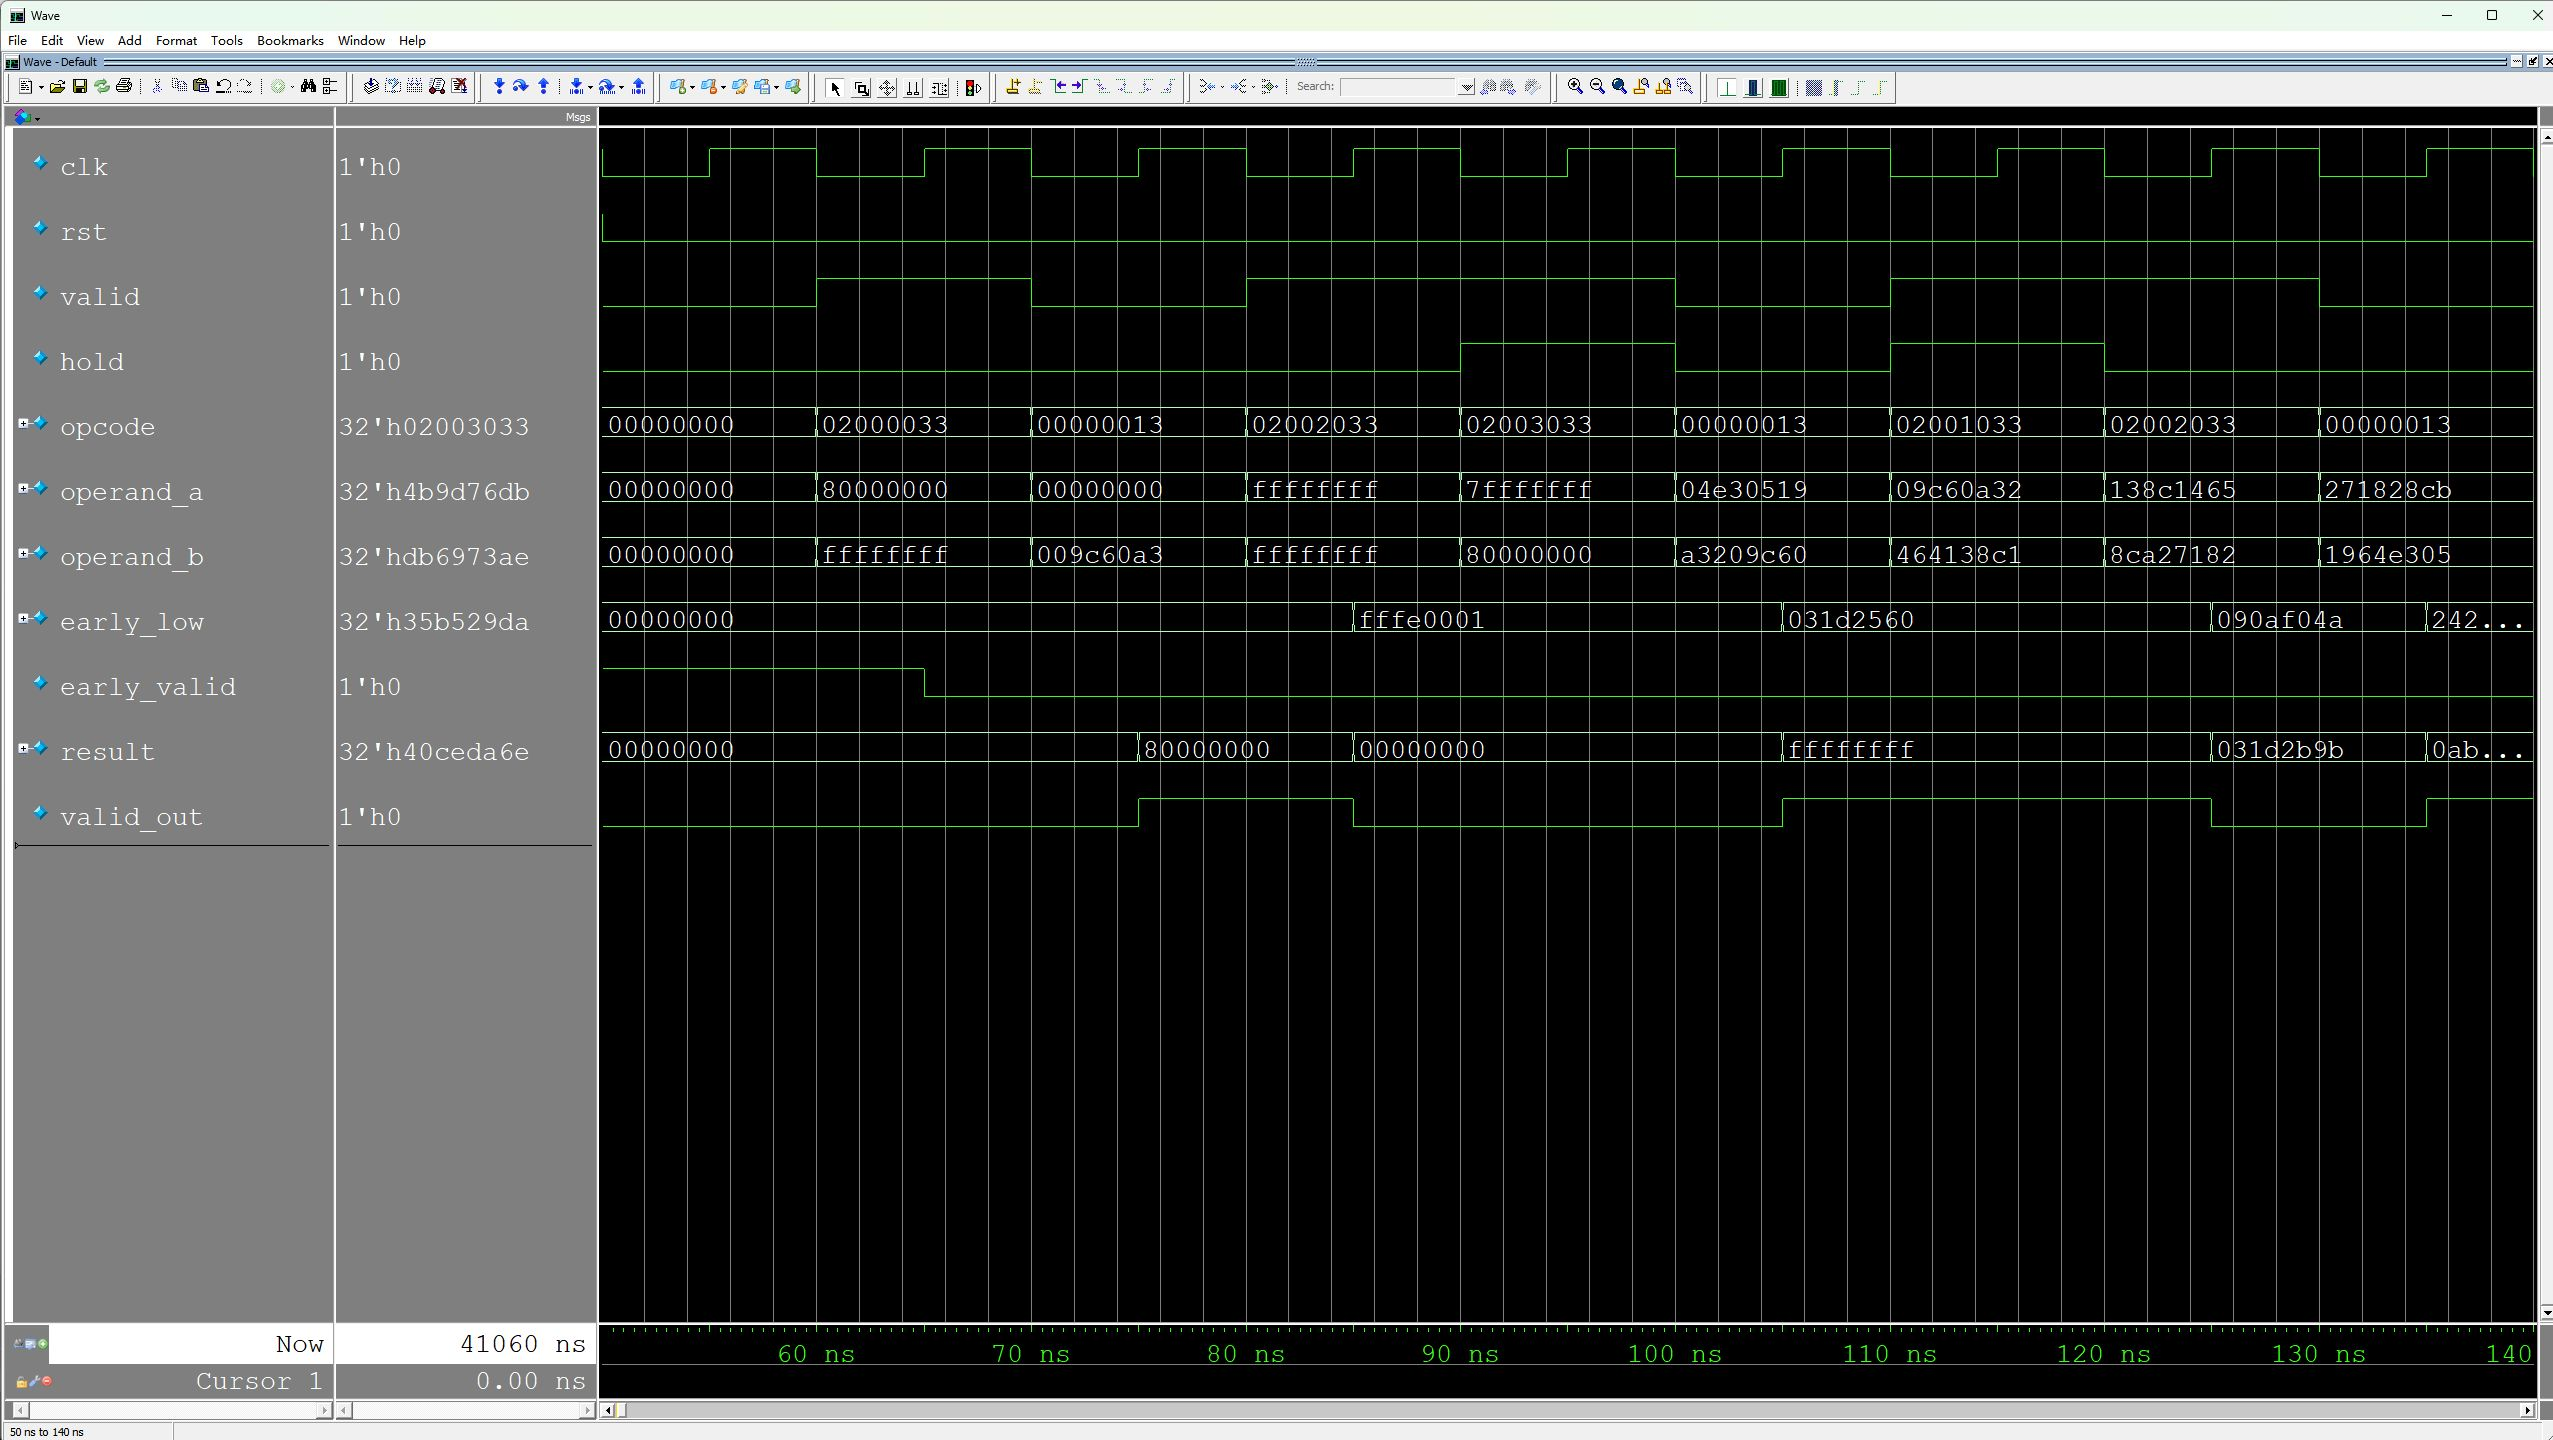
\includegraphics[width=0.8\linewidth]{../figure/cpu-unit-multiplier-modelsim-original.jpg}
\caption{乘法器的运算结果、无效气泡与暂停保持波形}
\label{fig:cpu-unit-multiplier}
\end{figure}

\subsubsection{除法器}

测试台按RISC-V除法规则独立计算商和余数，覆盖\texttt{DIV}、\texttt{DIVU}、\texttt{REM}和\texttt{REMU}。
除零时商为\texttt{0xFFFFFFFF}、余数为被除数；有符号最小值除以$-1$时，商为\texttt{0x80000000}、余数为零。
完成检查同时比较参考除法单元的结果，并核对当前单元相对参考单元延后一周期的完成时序。

图\ref{fig:cpu-unit-divider}给出$-21\div4$：输入为\texttt{0xFFFFFFEB}和\texttt{0x00000004}，输出商为\texttt{0xFFFFFFFB}（$-5$），符合向零截断规则。
首次操作经过迭代完成，随后再次提交相同操作数时利用保存的结果快速完成；两次\texttt{candidate\_valid}均比\texttt{golden\_valid}晚一个时钟周期。
算术测试完成308次操作；随后1000周期输入流继续覆盖忙时重启、连续有效输入和复位，累计检查312次完成事件。

\begin{figure}[!htbp]
\centering
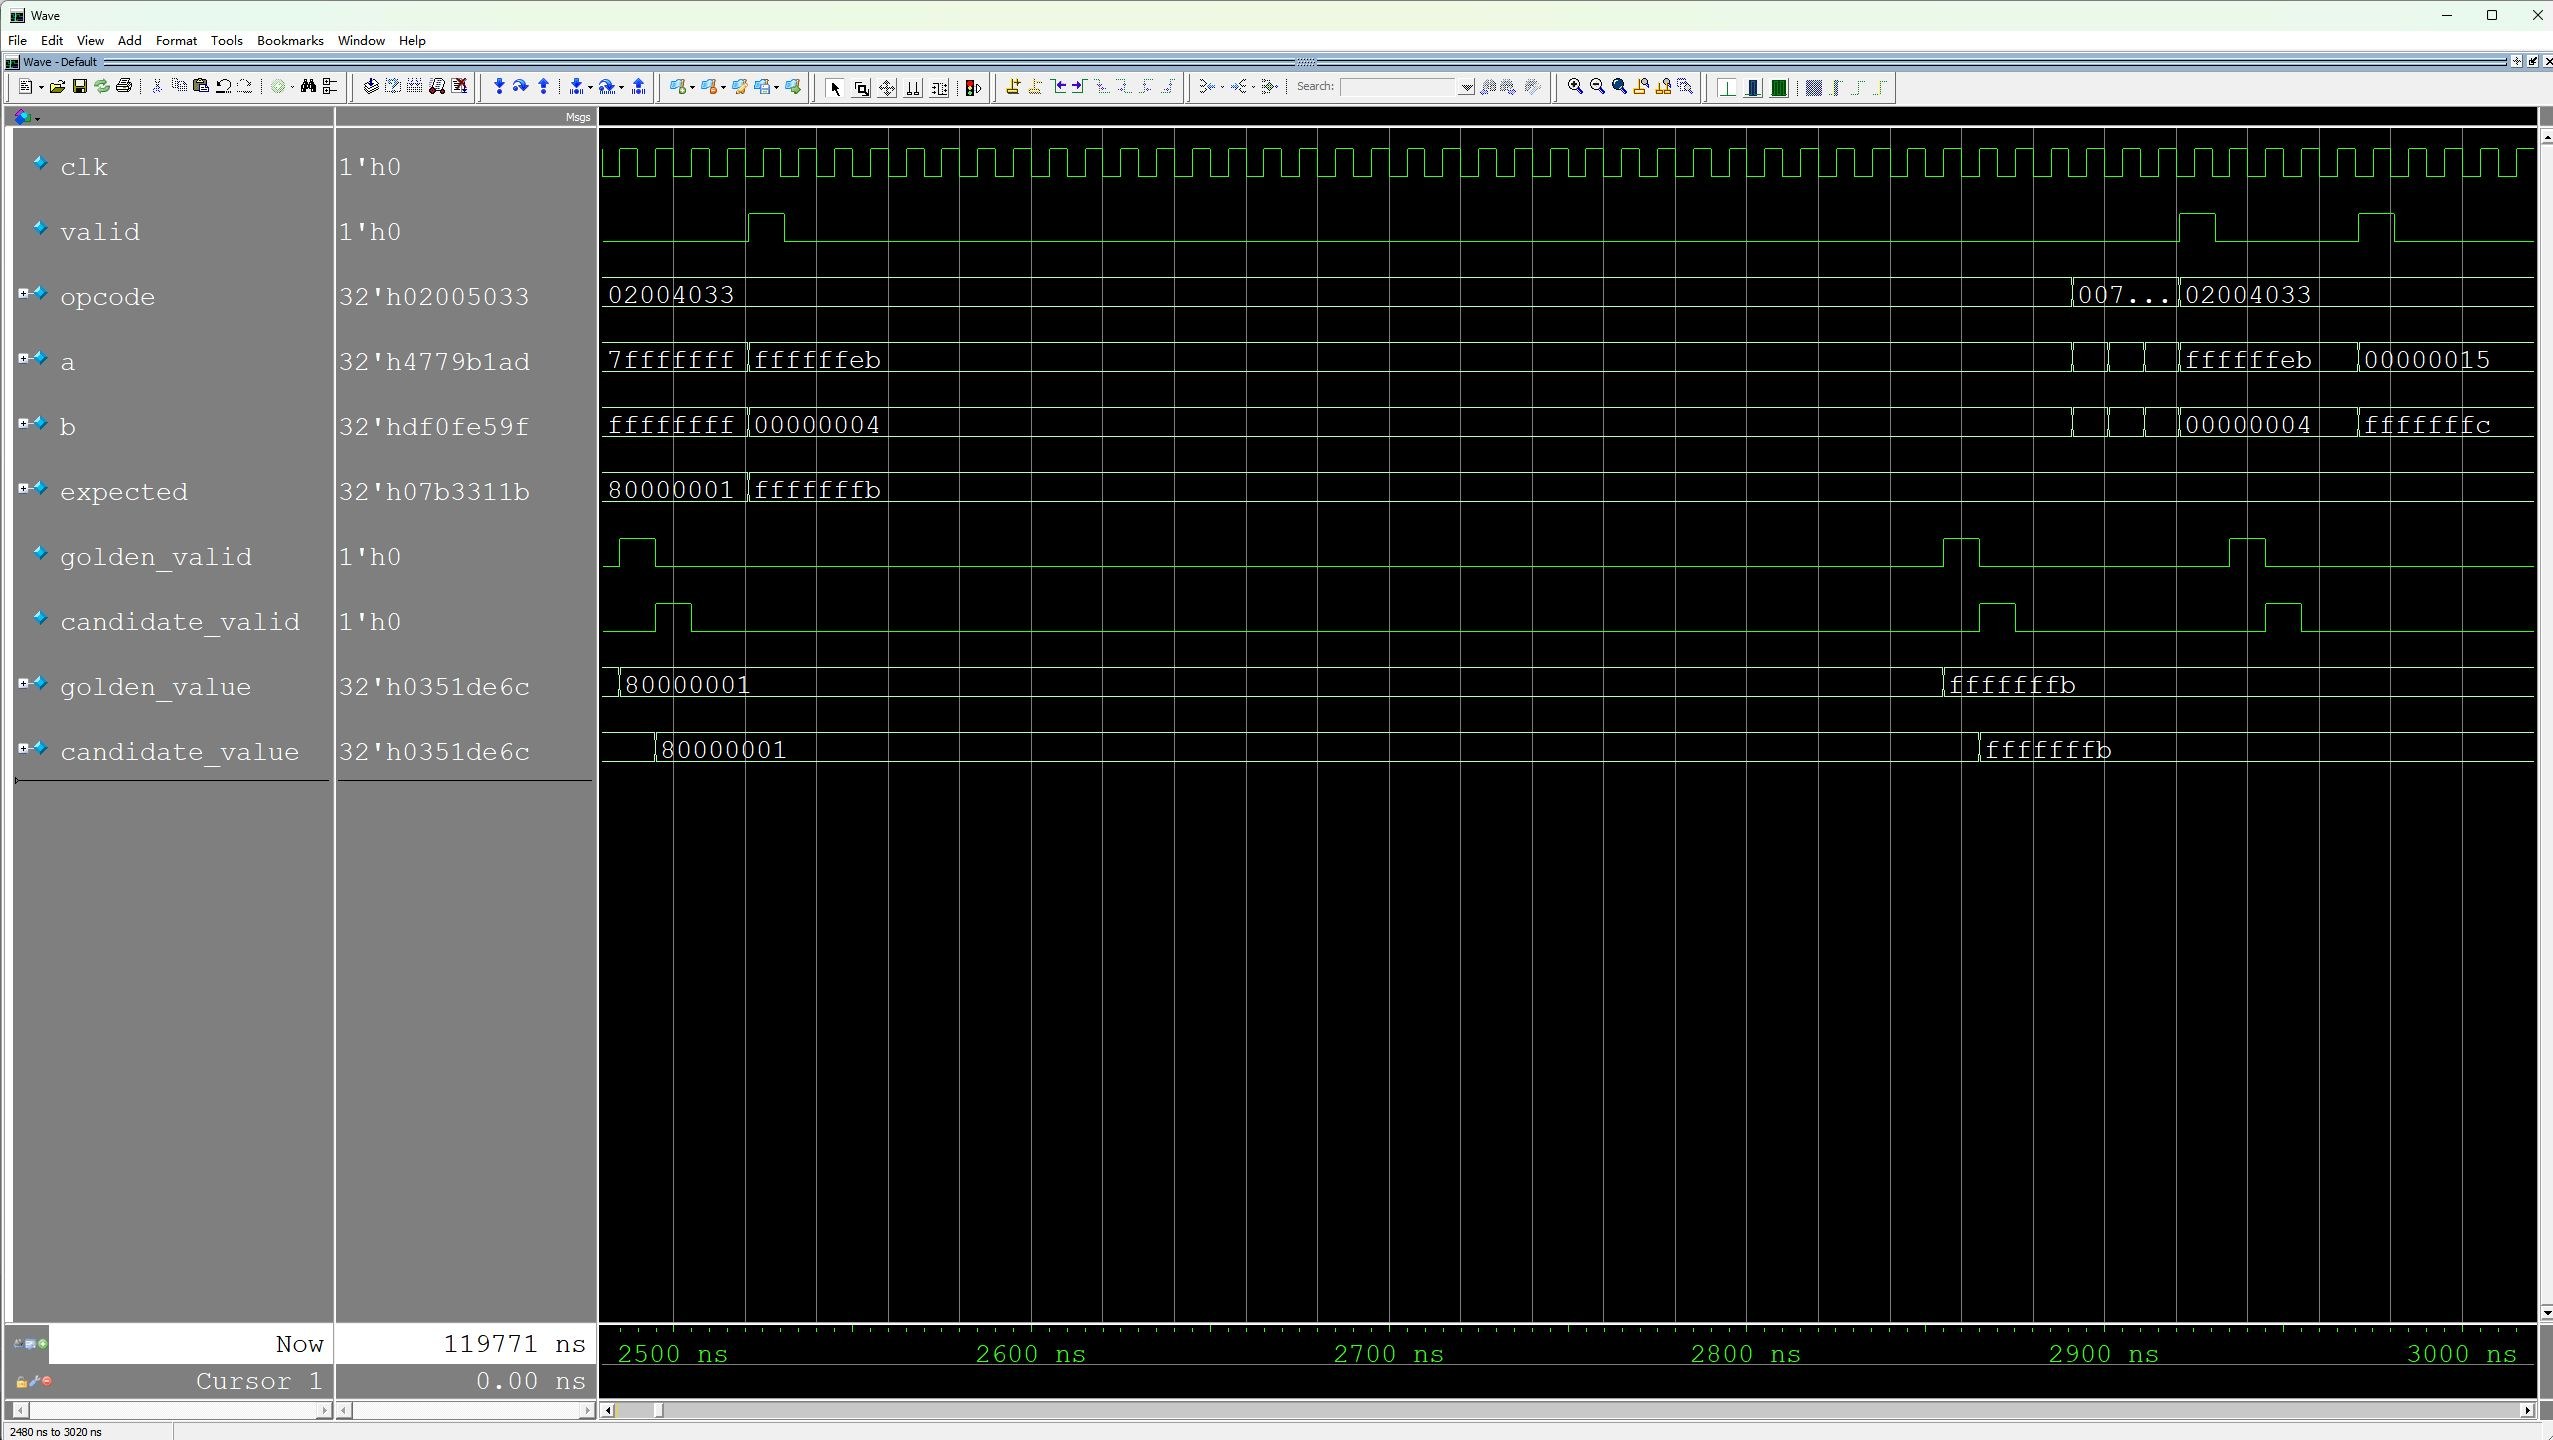
\includegraphics[width=0.8\linewidth]{../figure/cpu-unit-divider-modelsim-original.jpg}
\caption{有符号除法结果、完成时序及重复操作数复用波形}
\label{fig:cpu-unit-divider}
\end{figure}

\subsubsection{CSR}

测试台分别驱动指令输入与后续提交接口，检查CSR旧值、读改写结果和提交后的寄存器状态。
图\ref{fig:cpu-unit-csr}以\texttt{mscratch}（地址\texttt{0x340}）展示六种CSR指令：
先写入\texttt{0x12345678}，再用\texttt{0x00F0000F}置位得到\texttt{0x12F4567F}、清位得到\texttt{0x12045670}；
立即数交换、置位和清位依次得到\texttt{0x1F}、\texttt{0x1F}和\texttt{0x1C}。
\texttt{read\_valid}对应指令读值，\texttt{wb\_write}对应后续提交写入；\texttt{CSRRS}以\texttt{x0}为源寄存器时只读取旧值。

异常测试检查\texttt{mepc}低两位清零、非法指令的\texttt{mcause}=2与\texttt{mtval}、ECALL的\texttt{mcause}=11，以及异常入口和\texttt{MRET}的重定向地址与状态恢复。
自检完成21次CSR访问和91项检查，覆盖两次异常与一次返回。

\begin{figure}[!htbp]
\centering
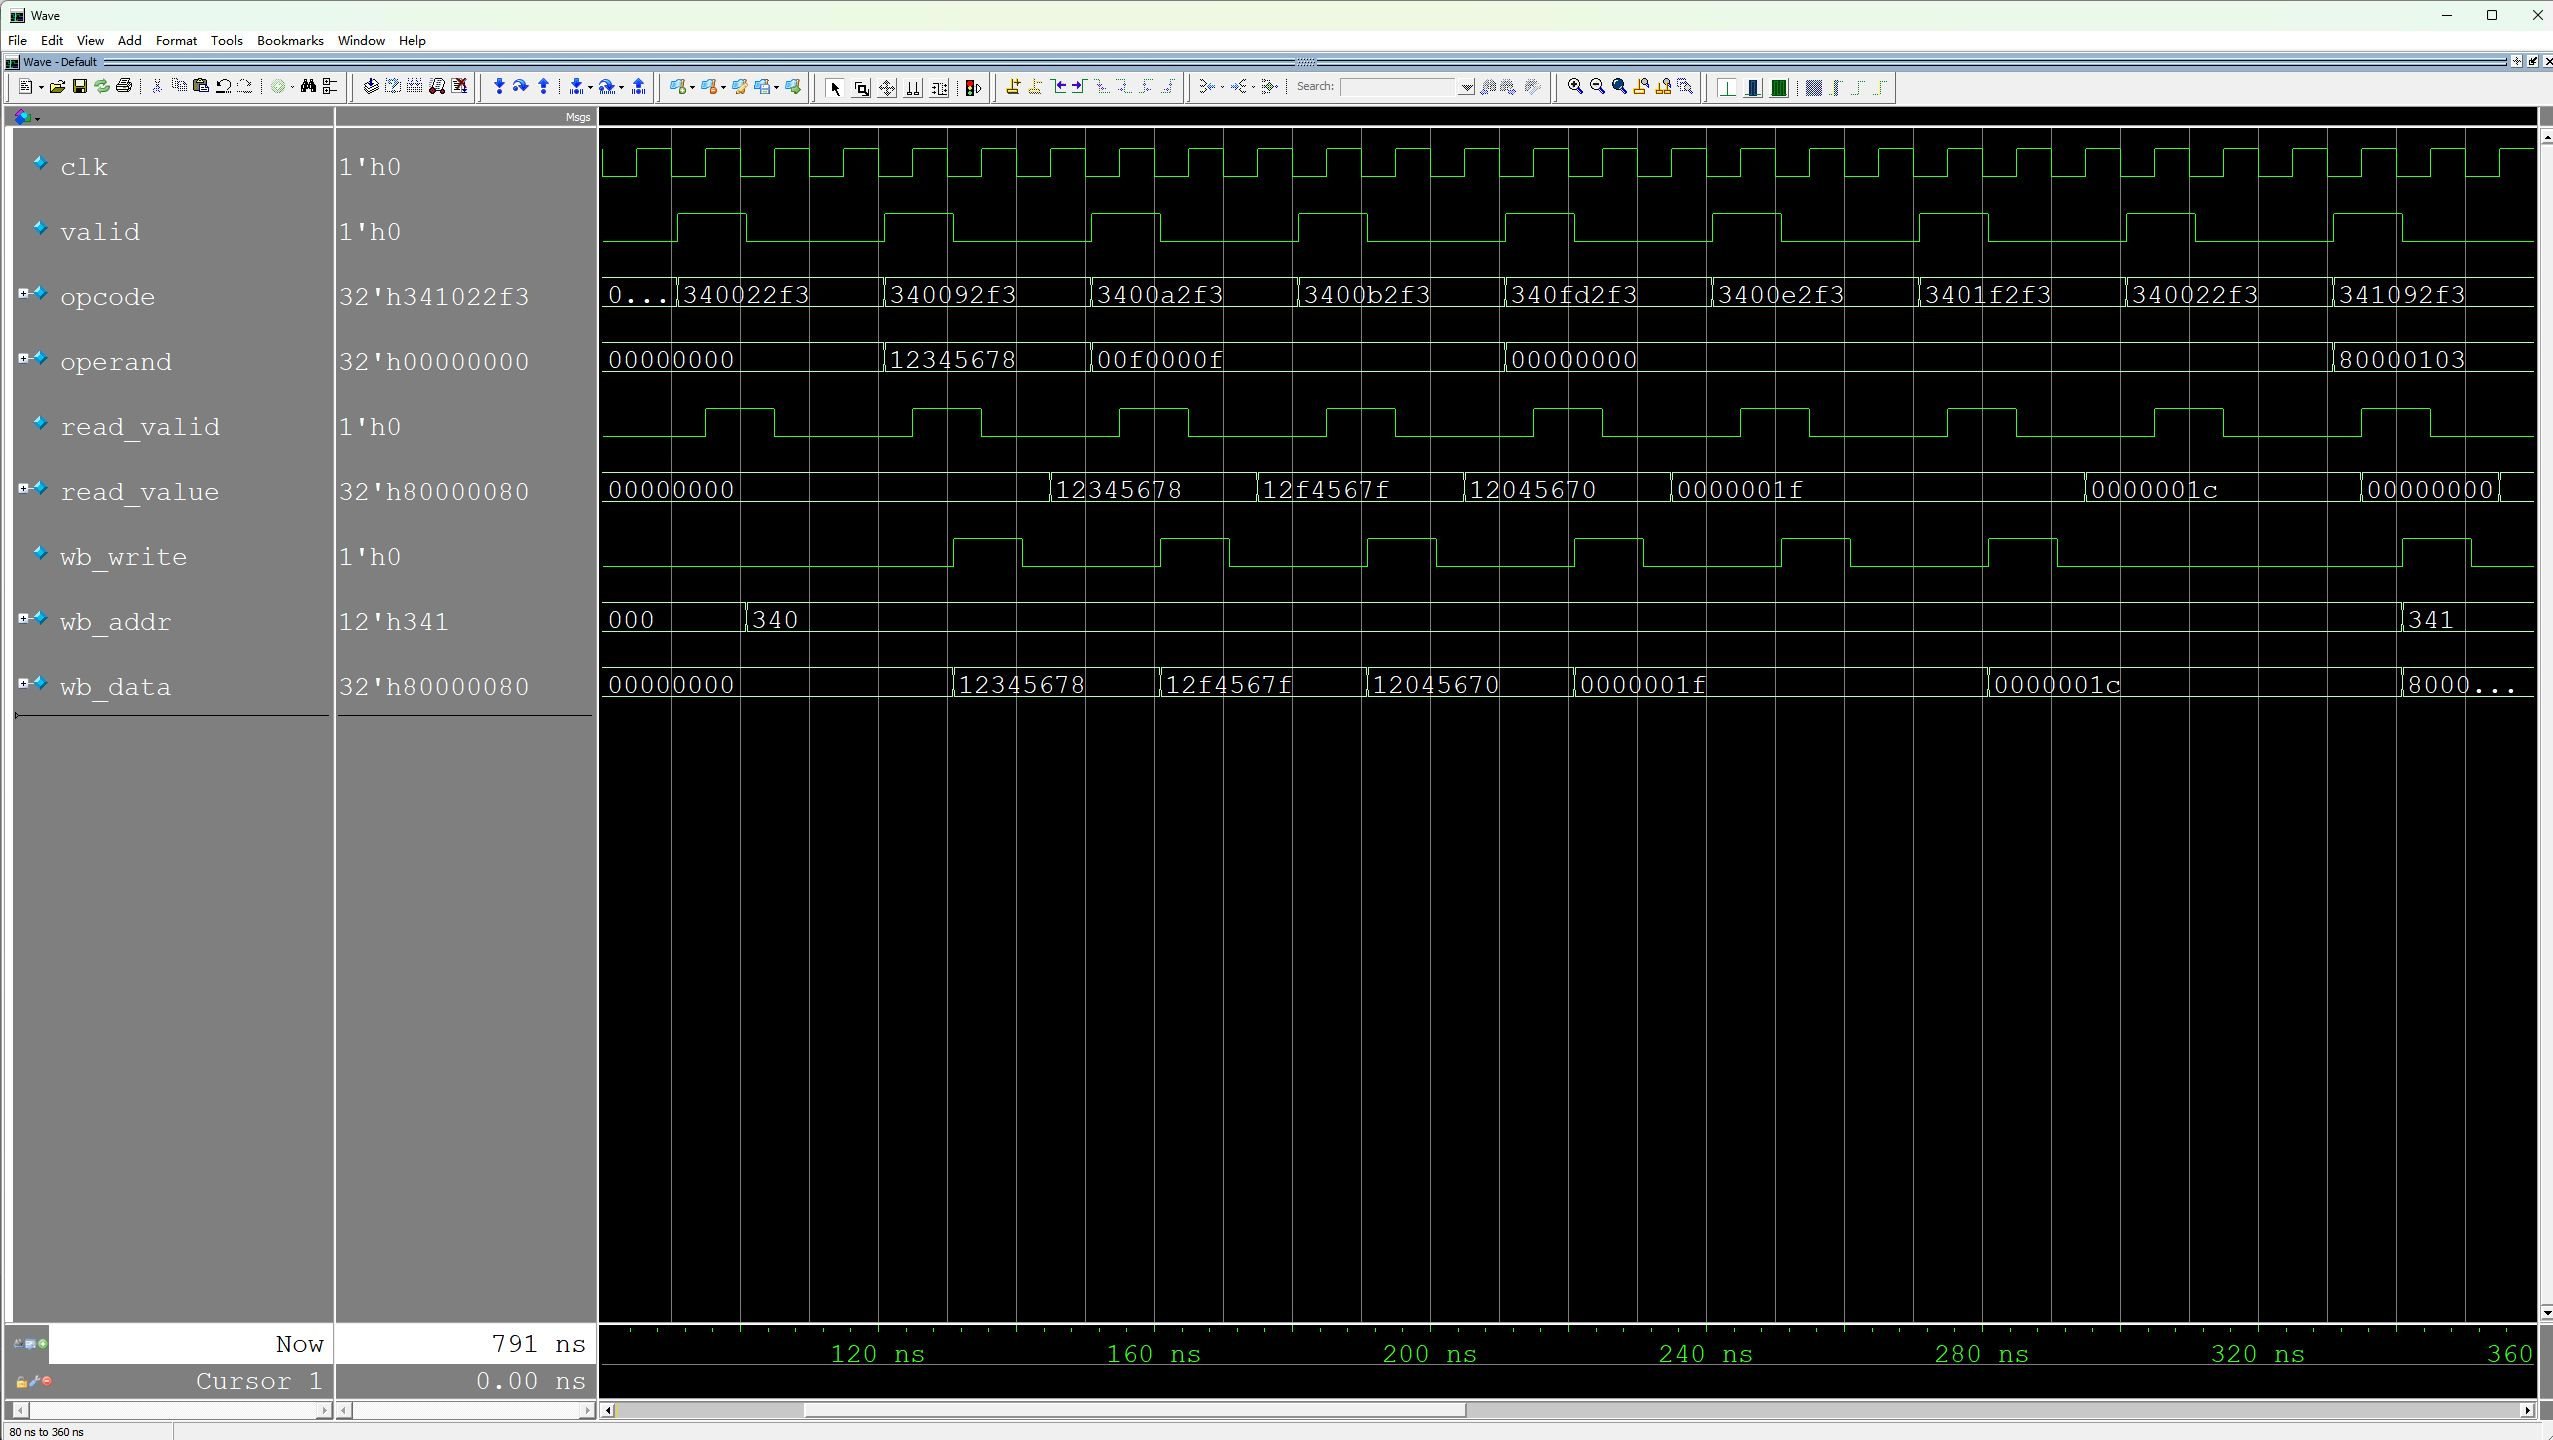
\includegraphics[width=0.8\linewidth]{../figure/cpu-unit-csr-modelsim-original.jpg}
\caption{CSR六种读改写形式的读值与提交写入波形}
\label{fig:cpu-unit-csr}
\end{figure}

CSR地址与中断优先级另由公开端口定向测试检查。主工程与CPU维护工作树分别运行6种参数组合，
覆盖机器模式与监督模式参数、生产编译与两种显式仿真控制配置，共12个实例、7916个检查点通过。
测试遍历MEI/MSI/MTI待决位的8种组合，检查机器中断优先级、外部中断输入及内部计时比较到期。
未实现CSR、只读CSR写入、零源只读访问、固定MISA和标准标识寄存器分别核对；
\texttt{0x7C1}至\texttt{0x7C3}检查命令编码、读回值、背压、成功和错误响应，旧PMP地址不再触发维护。

原ISA用例在维护版CSR实现上复跑，riscv-tests为50/50、ACT4为53/53通过，ELF和参考签名保持不变。
首轮102项通过、1项失败定位于标准标识CSR缺失；显式实现只读零后，该用例通过。
原失败、后续结果和输入哈希集中登记于\path{docs/verification/cpu/document_review_csr_20261102/}。
上述计数属于功能仿真，原板级资源、时序及CoreMark结果仍对应各自发布配置。

\subsubsection{ALU}

ALU结构见图\ref{fig:cpu-alu}。测试台对每个输入组合用独立的RV32参考函数计算结果，覆盖加法和减法的32位回绕、按位逻辑、无符号与有符号小于比较，以及逻辑左移、逻辑右移和算术右移。
边界集合包含零、全一、最高位、最高位减一、交替位和\texttt{0x80000001}；移位测试逐项检查0至31的移位量，并令移位操作数高位非零以检查只使用低5位。
图\ref{fig:cpu-unit-alu}中，\texttt{op}依次选择加法、移位、比较和逻辑运算，\texttt{expected}与\texttt{result}在每个检查窗口相同，\texttt{check\_ok}标记该组合已经完成比较。
测试还对1024组伪随机操作数执行全部16种控制编码，并覆盖默认操作的直通结果。

\begin{figure}[!htbp]
\centering
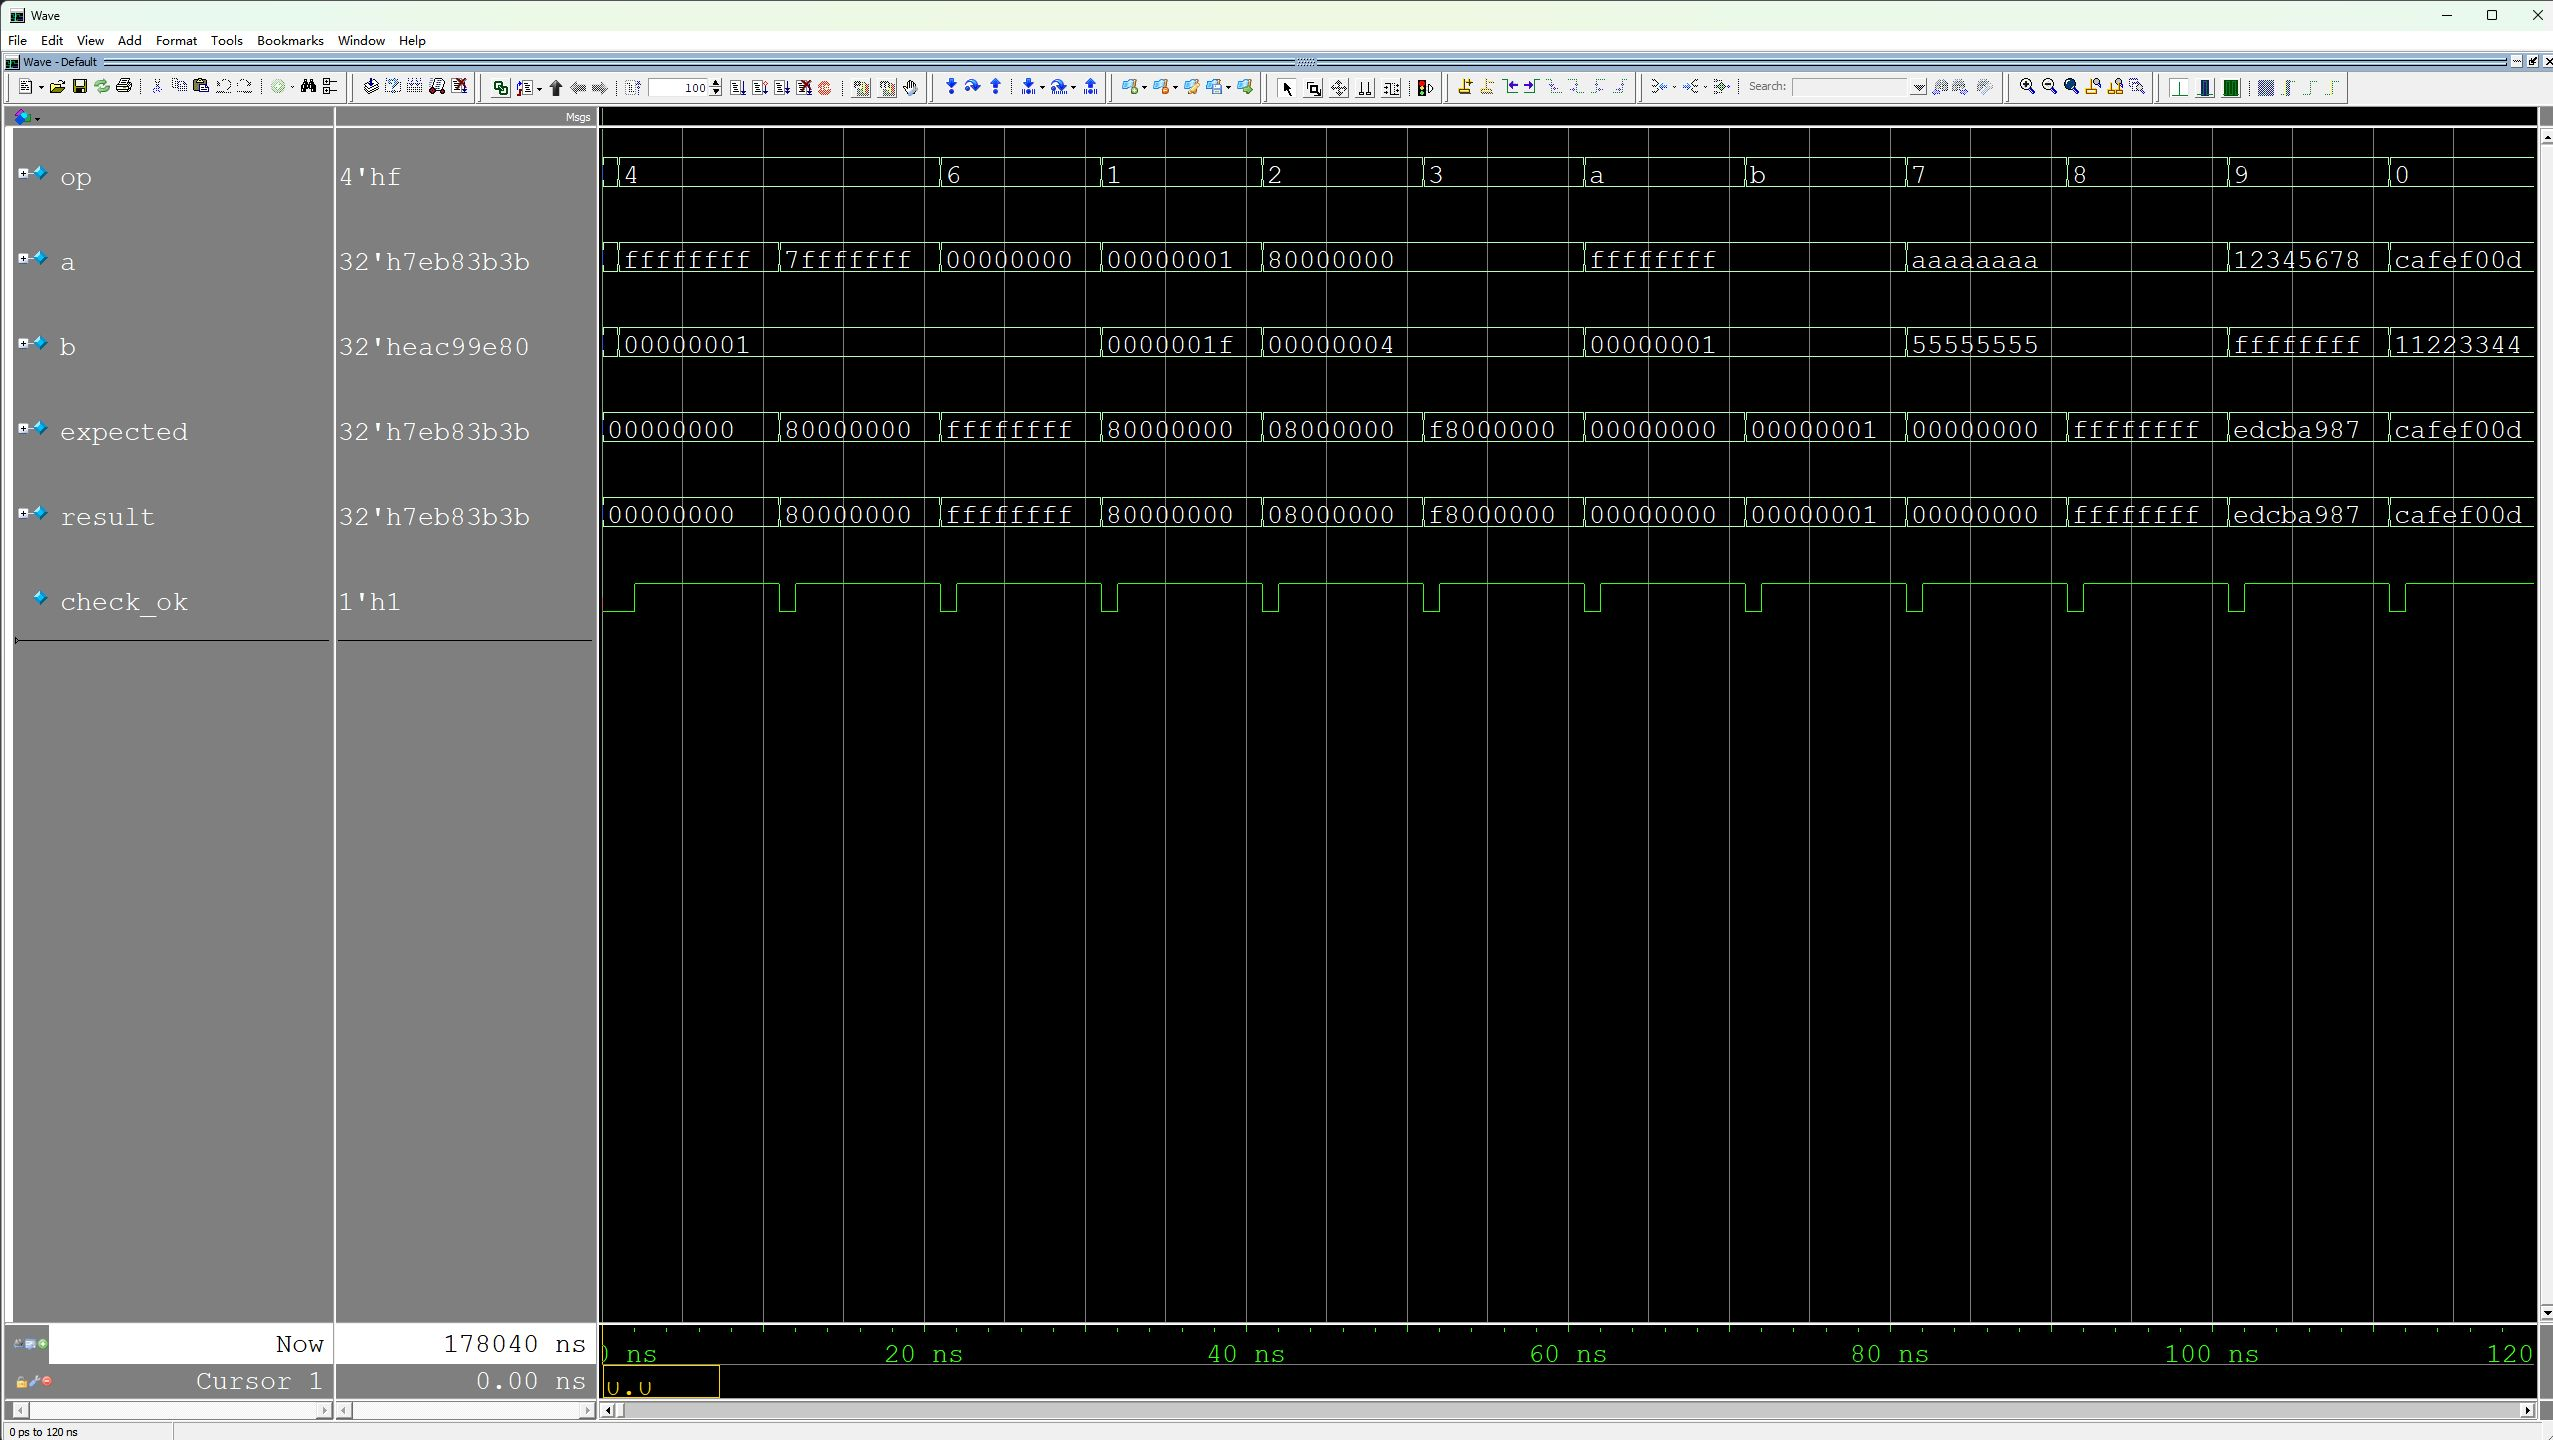
\includegraphics[width=0.8\linewidth]{../figure/cpu-unit-alu-modelsim-original.jpg}
\caption{ALU算术、移位、比较和逻辑运算结果波形}
\label{fig:cpu-unit-alu}
\end{figure}

\subsubsection{寄存器堆}

寄存器堆测试台以数组模型作为参考，按时钟上升沿更新写入，并在地址变化后立即比较两个异步读端口。
测试首先验证复位后的全部地址读为零，再逐字尝试写入32个寄存器；随后以伪随机地址和数据执行1000轮读写，并检查x0写入被丢弃。
单发射配置的次写口置零，测试台同时检查次读口输出为零。
图\ref{fig:cpu-unit-regfile}显示\texttt{rd}=5、6的写入在时钟边沿后分别出现在\texttt{value\_a}和\texttt{value\_b}，地址改变无需额外时钟即可读出；对x0的写入没有改变零值。
测试同时确认复位在时钟边沿后使全部地址读零，未在该边沿前提前改变读出数据；重写一个寄存器后，其余地址仍保持零值。

\begin{figure}[!htbp]
\centering
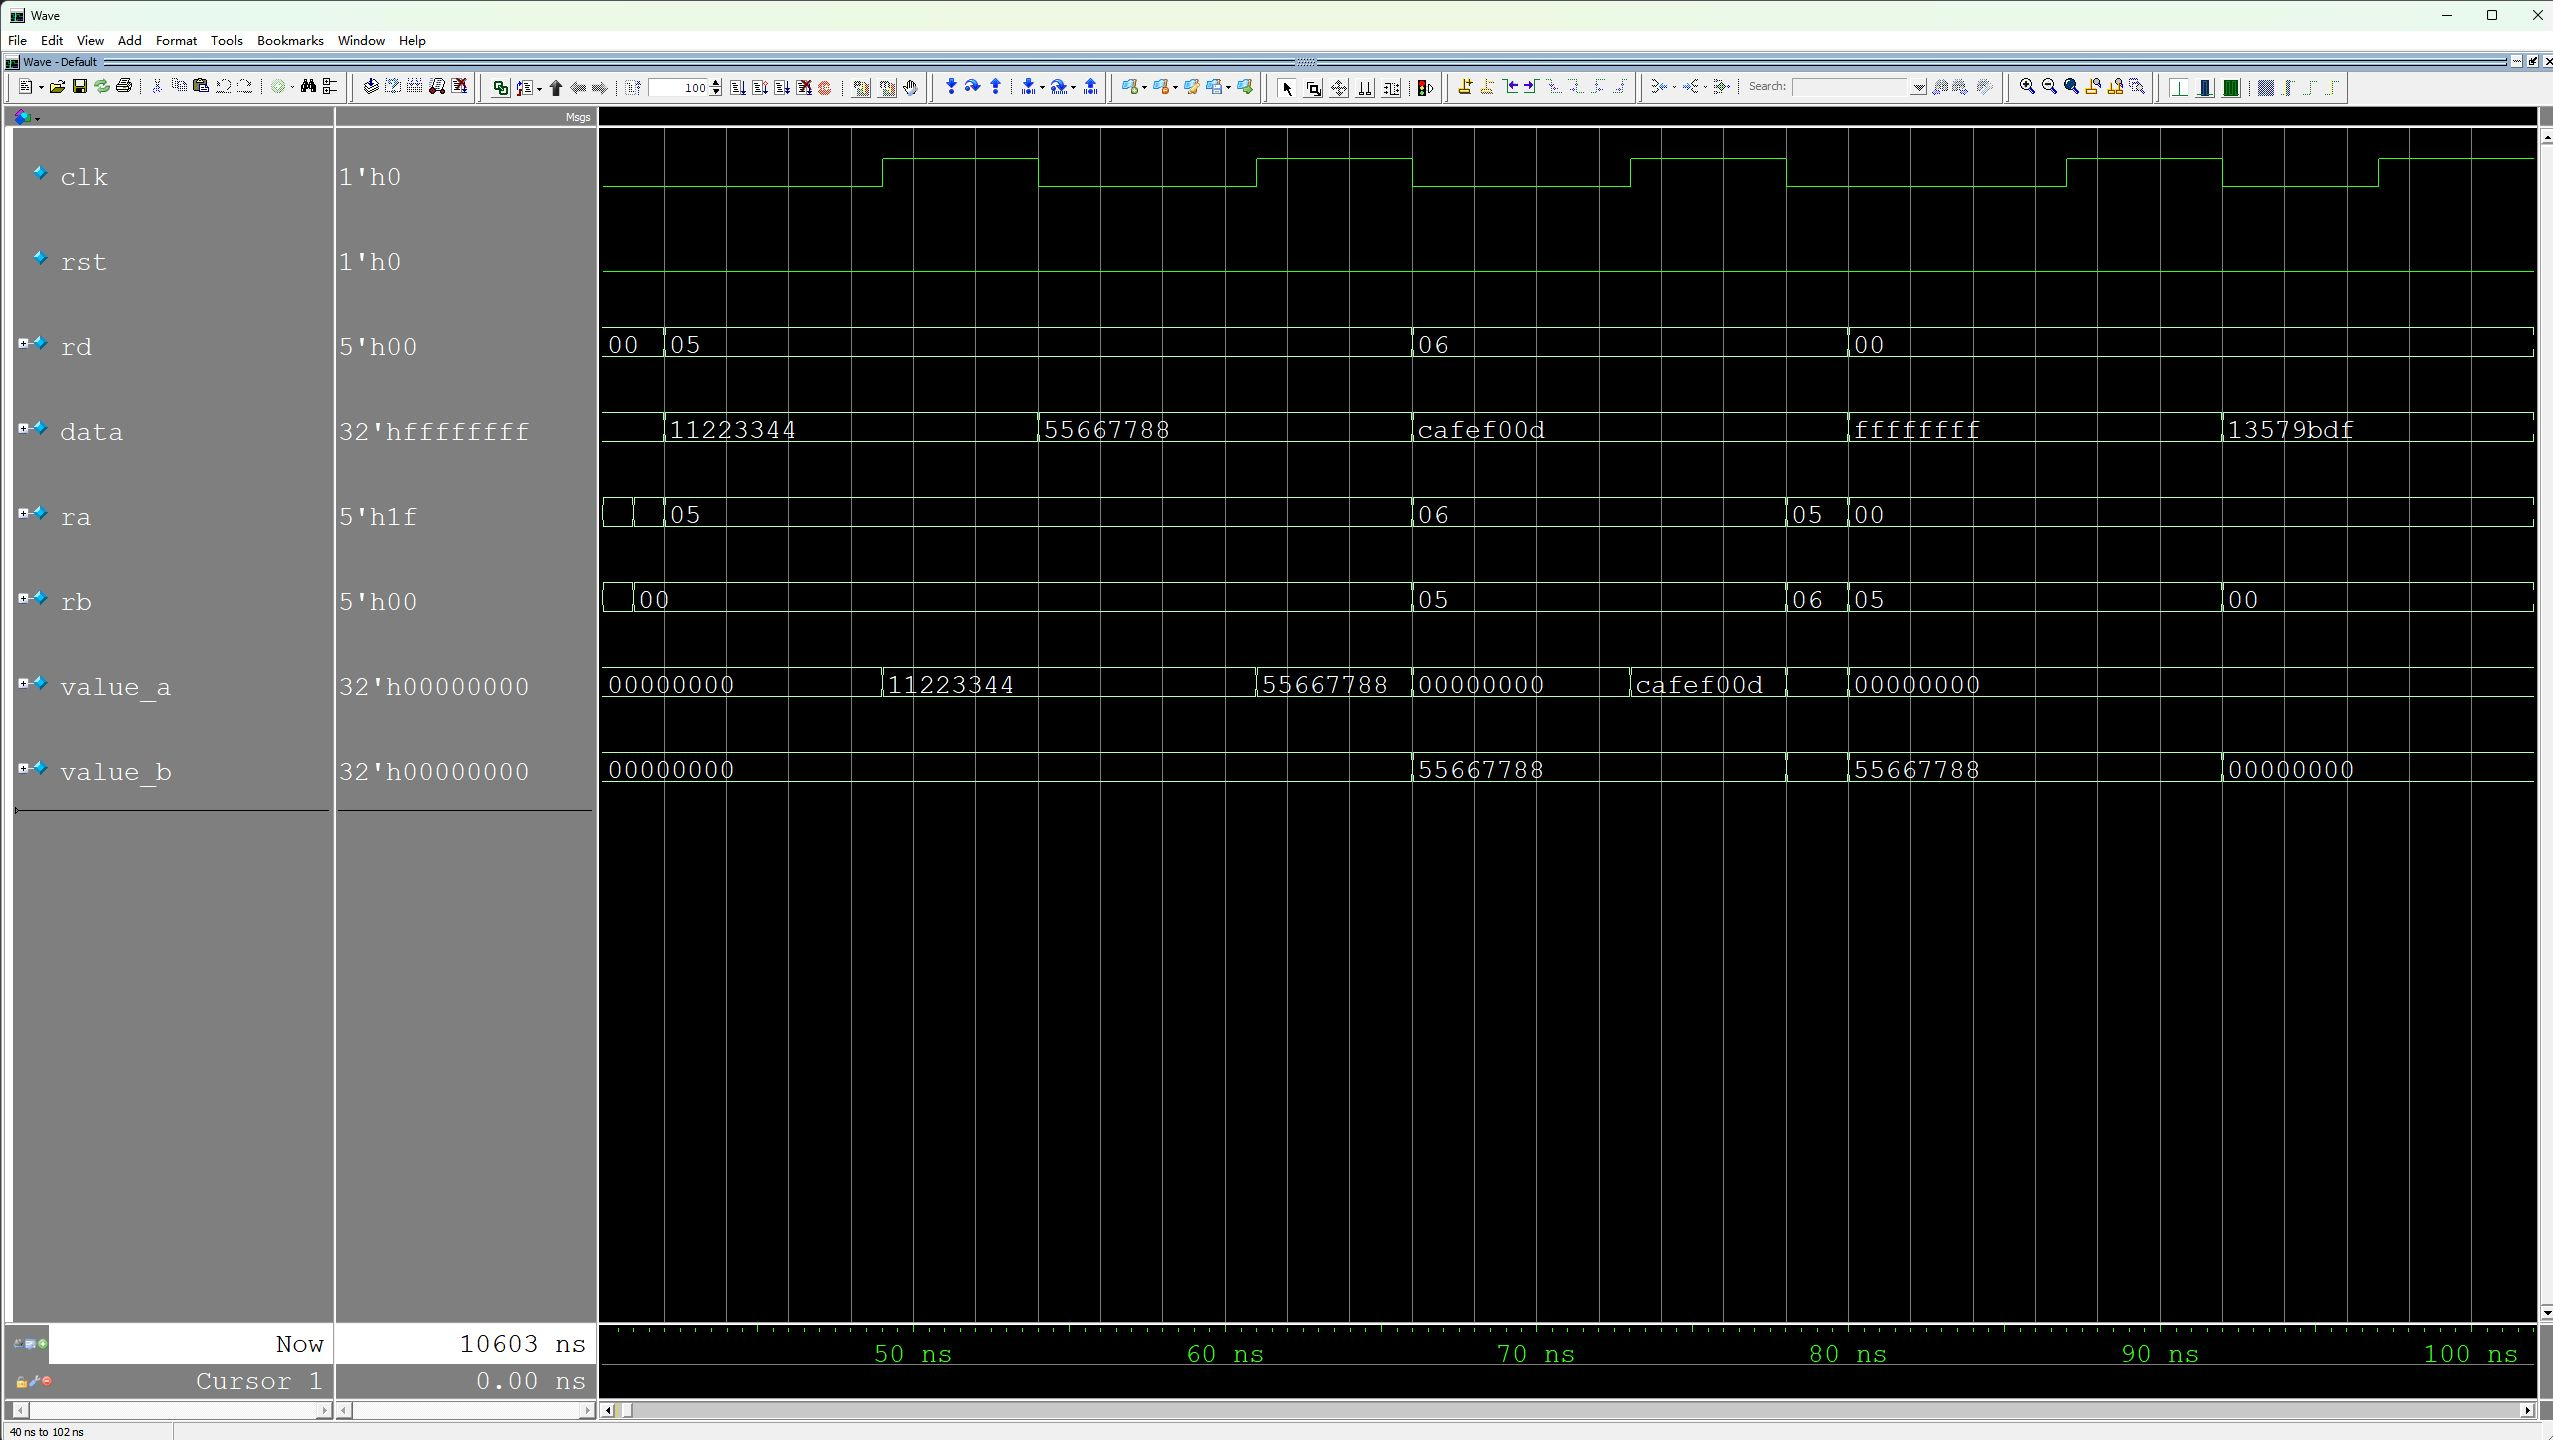
\includegraphics[width=0.8\linewidth]{../figure/cpu-unit-regfile-modelsim-original.jpg}
\caption{寄存器堆同步写入、异步读出及x0保持波形}
\label{fig:cpu-unit-regfile}
\end{figure}

\subsection{模块级仿真验证}

模块级测试覆盖前端重定向、发射与旁路、LSU和I/D Cache，自检结果见表\ref{tbl:cpu-module-results}。
前端测试在取指请求接纳、响应返回和指令输出握手处注入延迟，发射测试通过完整核的取指和数据接口运行固定指令序列；LSU与Cache测试分别连接各自的请求和响应端口。
结果、自检日志、WLF/VCD和截图集中保存于\path{docs/verification/cpu/module_support/}。

\begin{reporttable}
\begin{longtable}{@{}p{0.15\linewidth}p{0.40\linewidth}p{0.28\linewidth}p{0.08\linewidth}@{}}
\caption{CPU模块级功能仿真结果}\label{tbl:cpu-module-results}\\
\toprule
模块 & 场景 & 检查统计 & 结果 \\
\midrule
\endfirsthead
\caption[]{CPU模块级功能仿真结果（续）}\\
\toprule
模块 & 场景 & 检查统计 & 结果 \\
\midrule
\endhead
\bottomrule
\endfoot
前端重定向 & 重定向请求寄存、迟到取指响应、接收端背压和连续重定向 & 4次重定向，12项有效指令输出，4项迟到响应丢弃 & PASS \\
发射/旁路 & 连续ALU、加载、低位乘法、高位乘法和同目的寄存器写回 & 16次发射，16次退休，26项操作数检查，38周期 & PASS \\
LSU & 加载扩展、写掩码、请求保持、非对齐和总线错误 & 18次访问，220/220项检查 & PASS \\
I/D Cache & 命中、填充、两路替换、错误填充、维护及并发 & 1297/1297项检查 & PASS \\
数据Cache写回 & 脏行清理、失败重试、替换、刷新与共享区旁路 & 1355/1355项检查 & PASS \\
数据Cache响应重叠 & 连续命中、响应标签、后续请求及错误隔离 & 142/142项检查，12次连续读取 & PASS \\
\end{longtable}
\end{reporttable}

\subsubsection{前端重定向}

测试台关闭动态分支预测，使用固定32\,bit指令返回，分别设置取指返回延迟、接收端暂停和分支目标。
重定向请求在时钟边沿登记，旧取指响应在返回时丢弃；恢复后，接收端只接纳从目标地址开始的低字和高字。
图\ref{fig:cpu-module-frontend}中，\texttt{branch}在目标\texttt{0x80001000}和\texttt{0x80002000}处触发，\texttt{pending}覆盖等待窗口，\texttt{response}晚于请求返回，\texttt{dropped}累计迟到响应；\texttt{pc0}保持目标序列，未输出旧地址指令。
测试完成4次重定向、12项正确指令输出和4项迟到响应丢弃。

\begin{figure}[htbp]
\centering
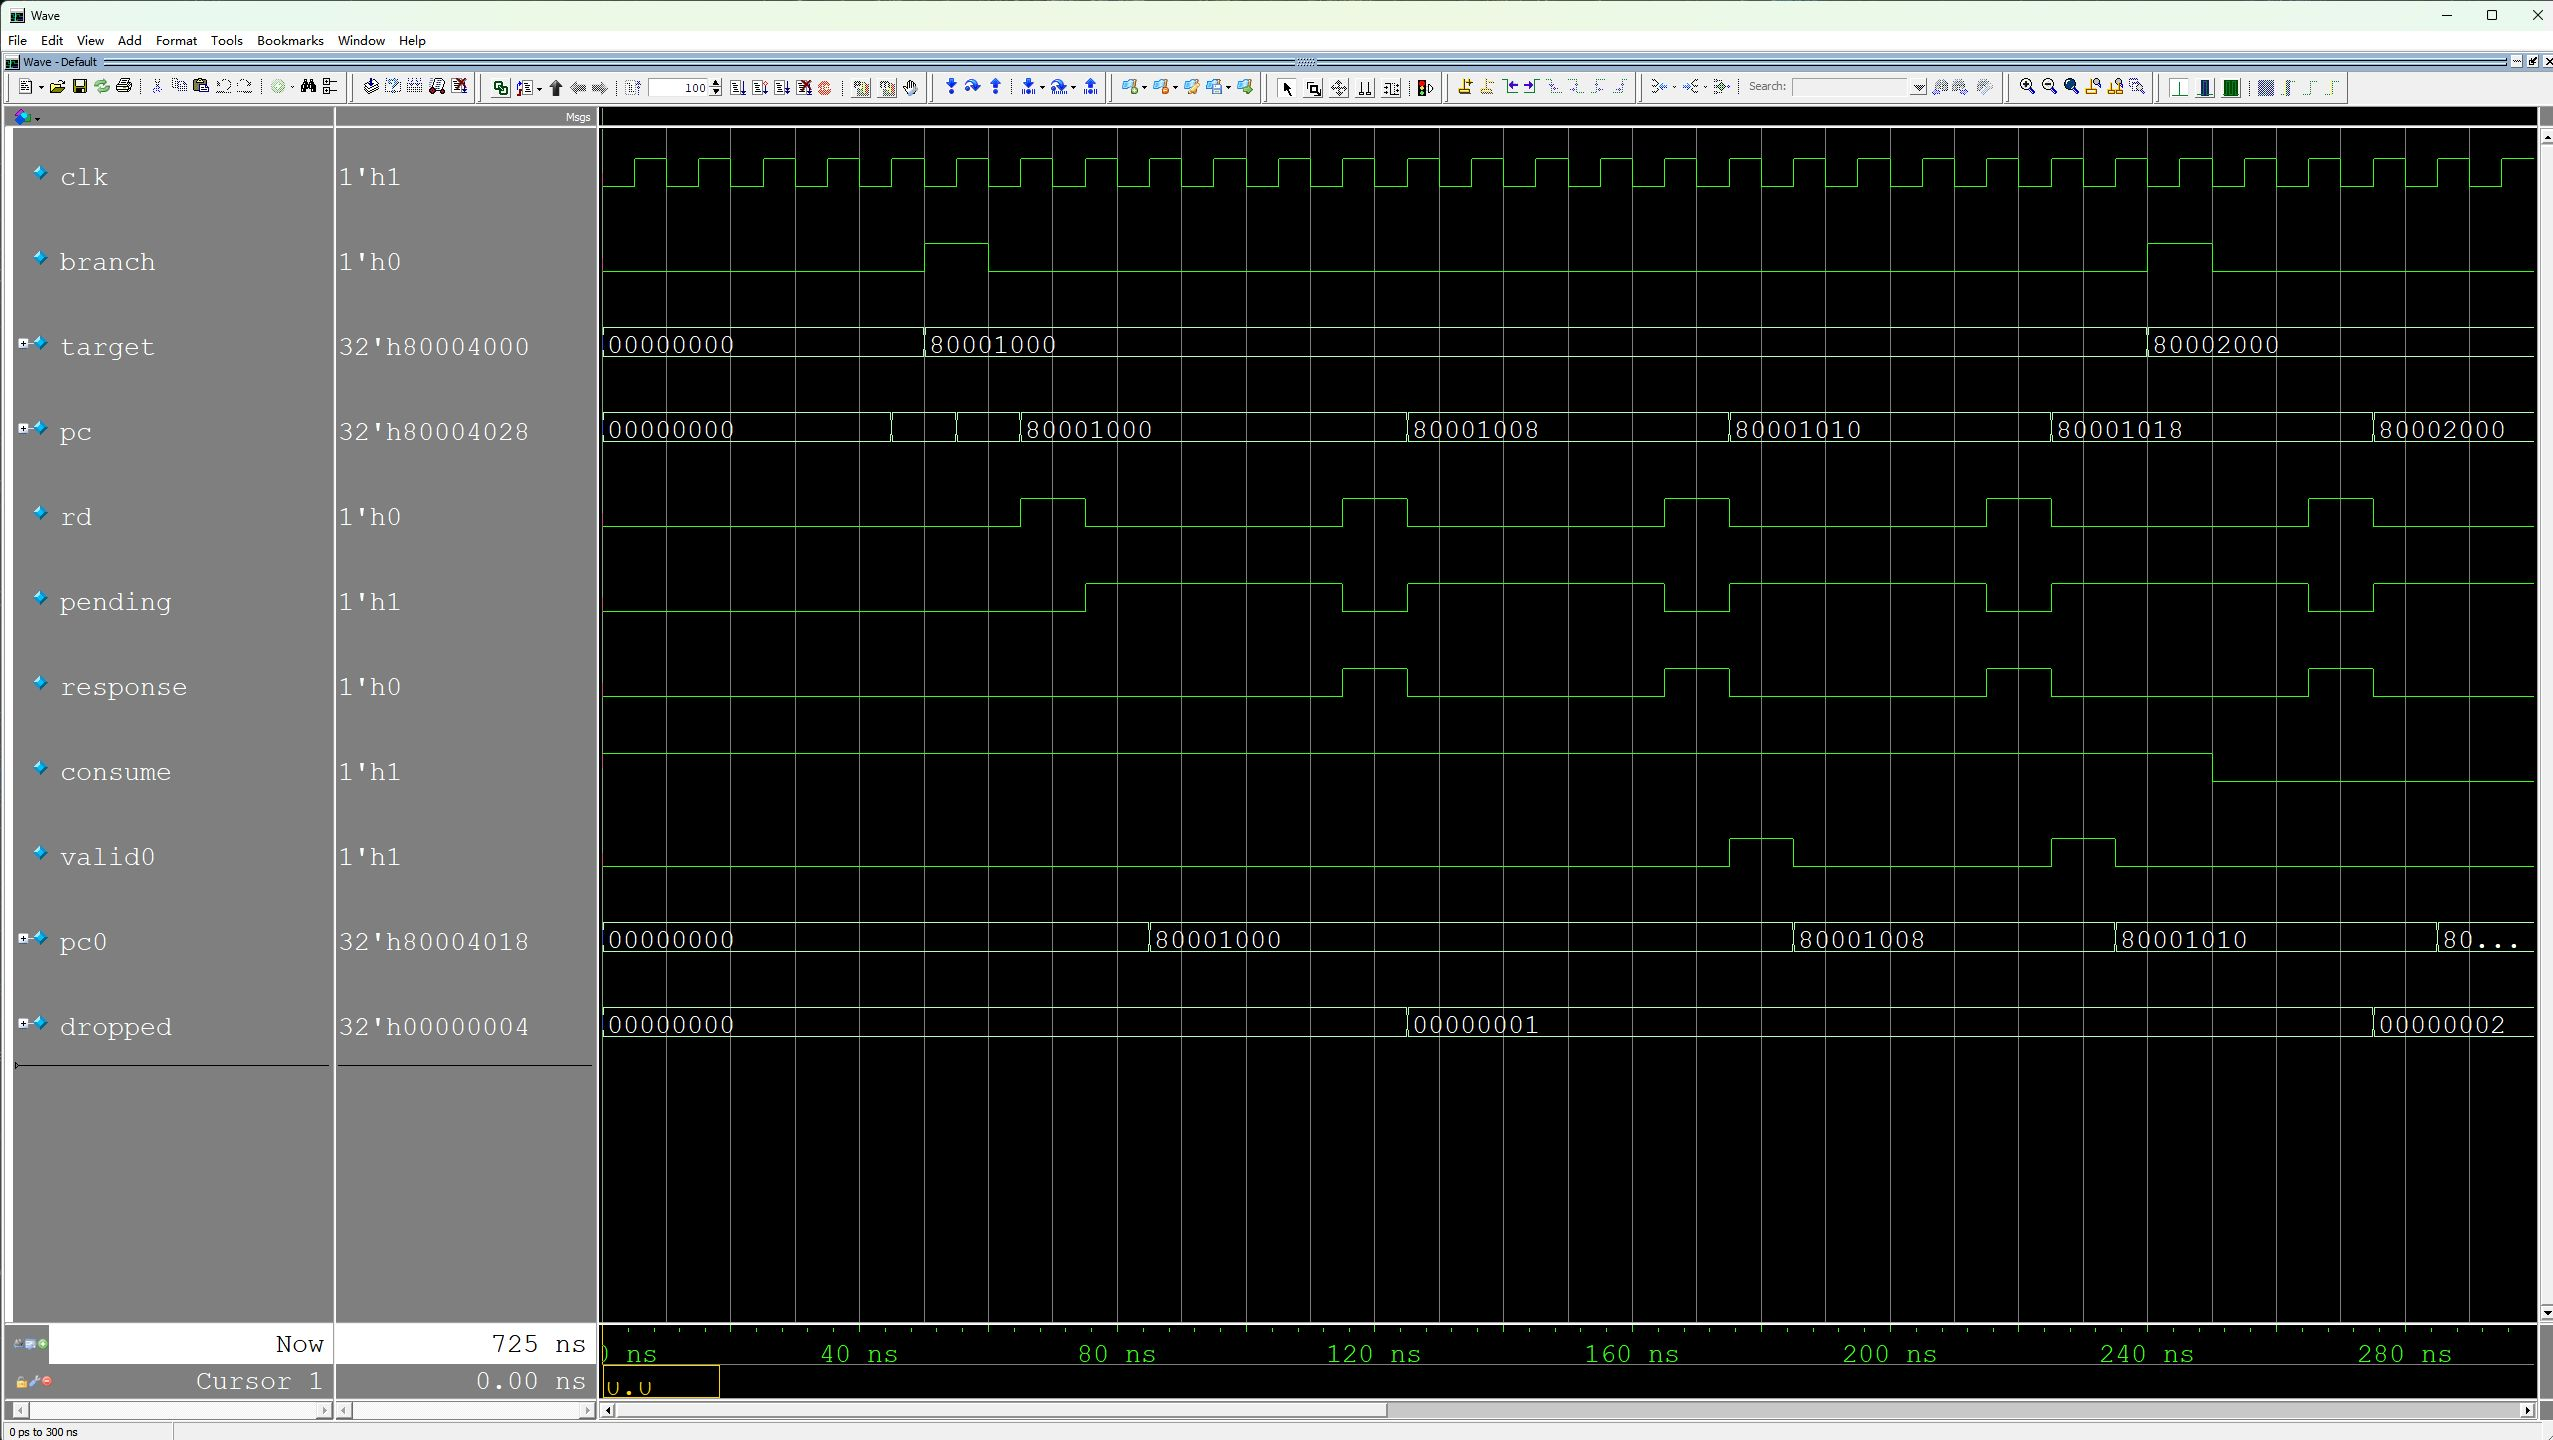
\includegraphics[width=0.8\linewidth]{../figure/cpu-module-frontend-redirect-modelsim-original.jpg}
\caption{前端重定向请求寄存、迟到响应丢弃和目标指令输出波形}
\label{fig:cpu-module-frontend}
\end{figure}

\subsubsection{发射与旁路}

测试台通过真实指令取指返回运行16条顺序指令，包含连续加法、一次加载、低位乘法、高位乘法和两次写入同一目的寄存器。
数据端口在接纳请求前插入等待，并推迟加载返回；测试检查相关指令在数据可用后发射，高位乘法保持互锁，满足条件的低位乘法使用E1早期旁路。
连续两条指令写入同一目的寄存器时，下一条相关指令必须读取较新结果。
图\ref{fig:cpu-module-issueflow}中，\texttt{d\_rd}、\texttt{d\_accept}和\texttt{d\_ack}形成一次完整加载事务；\texttt{load\_e1/load\_e2}和\texttt{pipe\_stall}标出等待区间，\texttt{mul\_e1/early\_mul}标出低位乘法旁路，\texttt{wb\_valid/wb\_pc}保持顺序退休。
自检在38个周期内完成16次发射和16次退休，检查26个操作数，记录10个加载相关等待周期和1个高位乘法等待周期；ALU E1旁路、低位乘法早旁路和最新结果优先级各命中一次。

\begin{figure}[htbp]
\centering
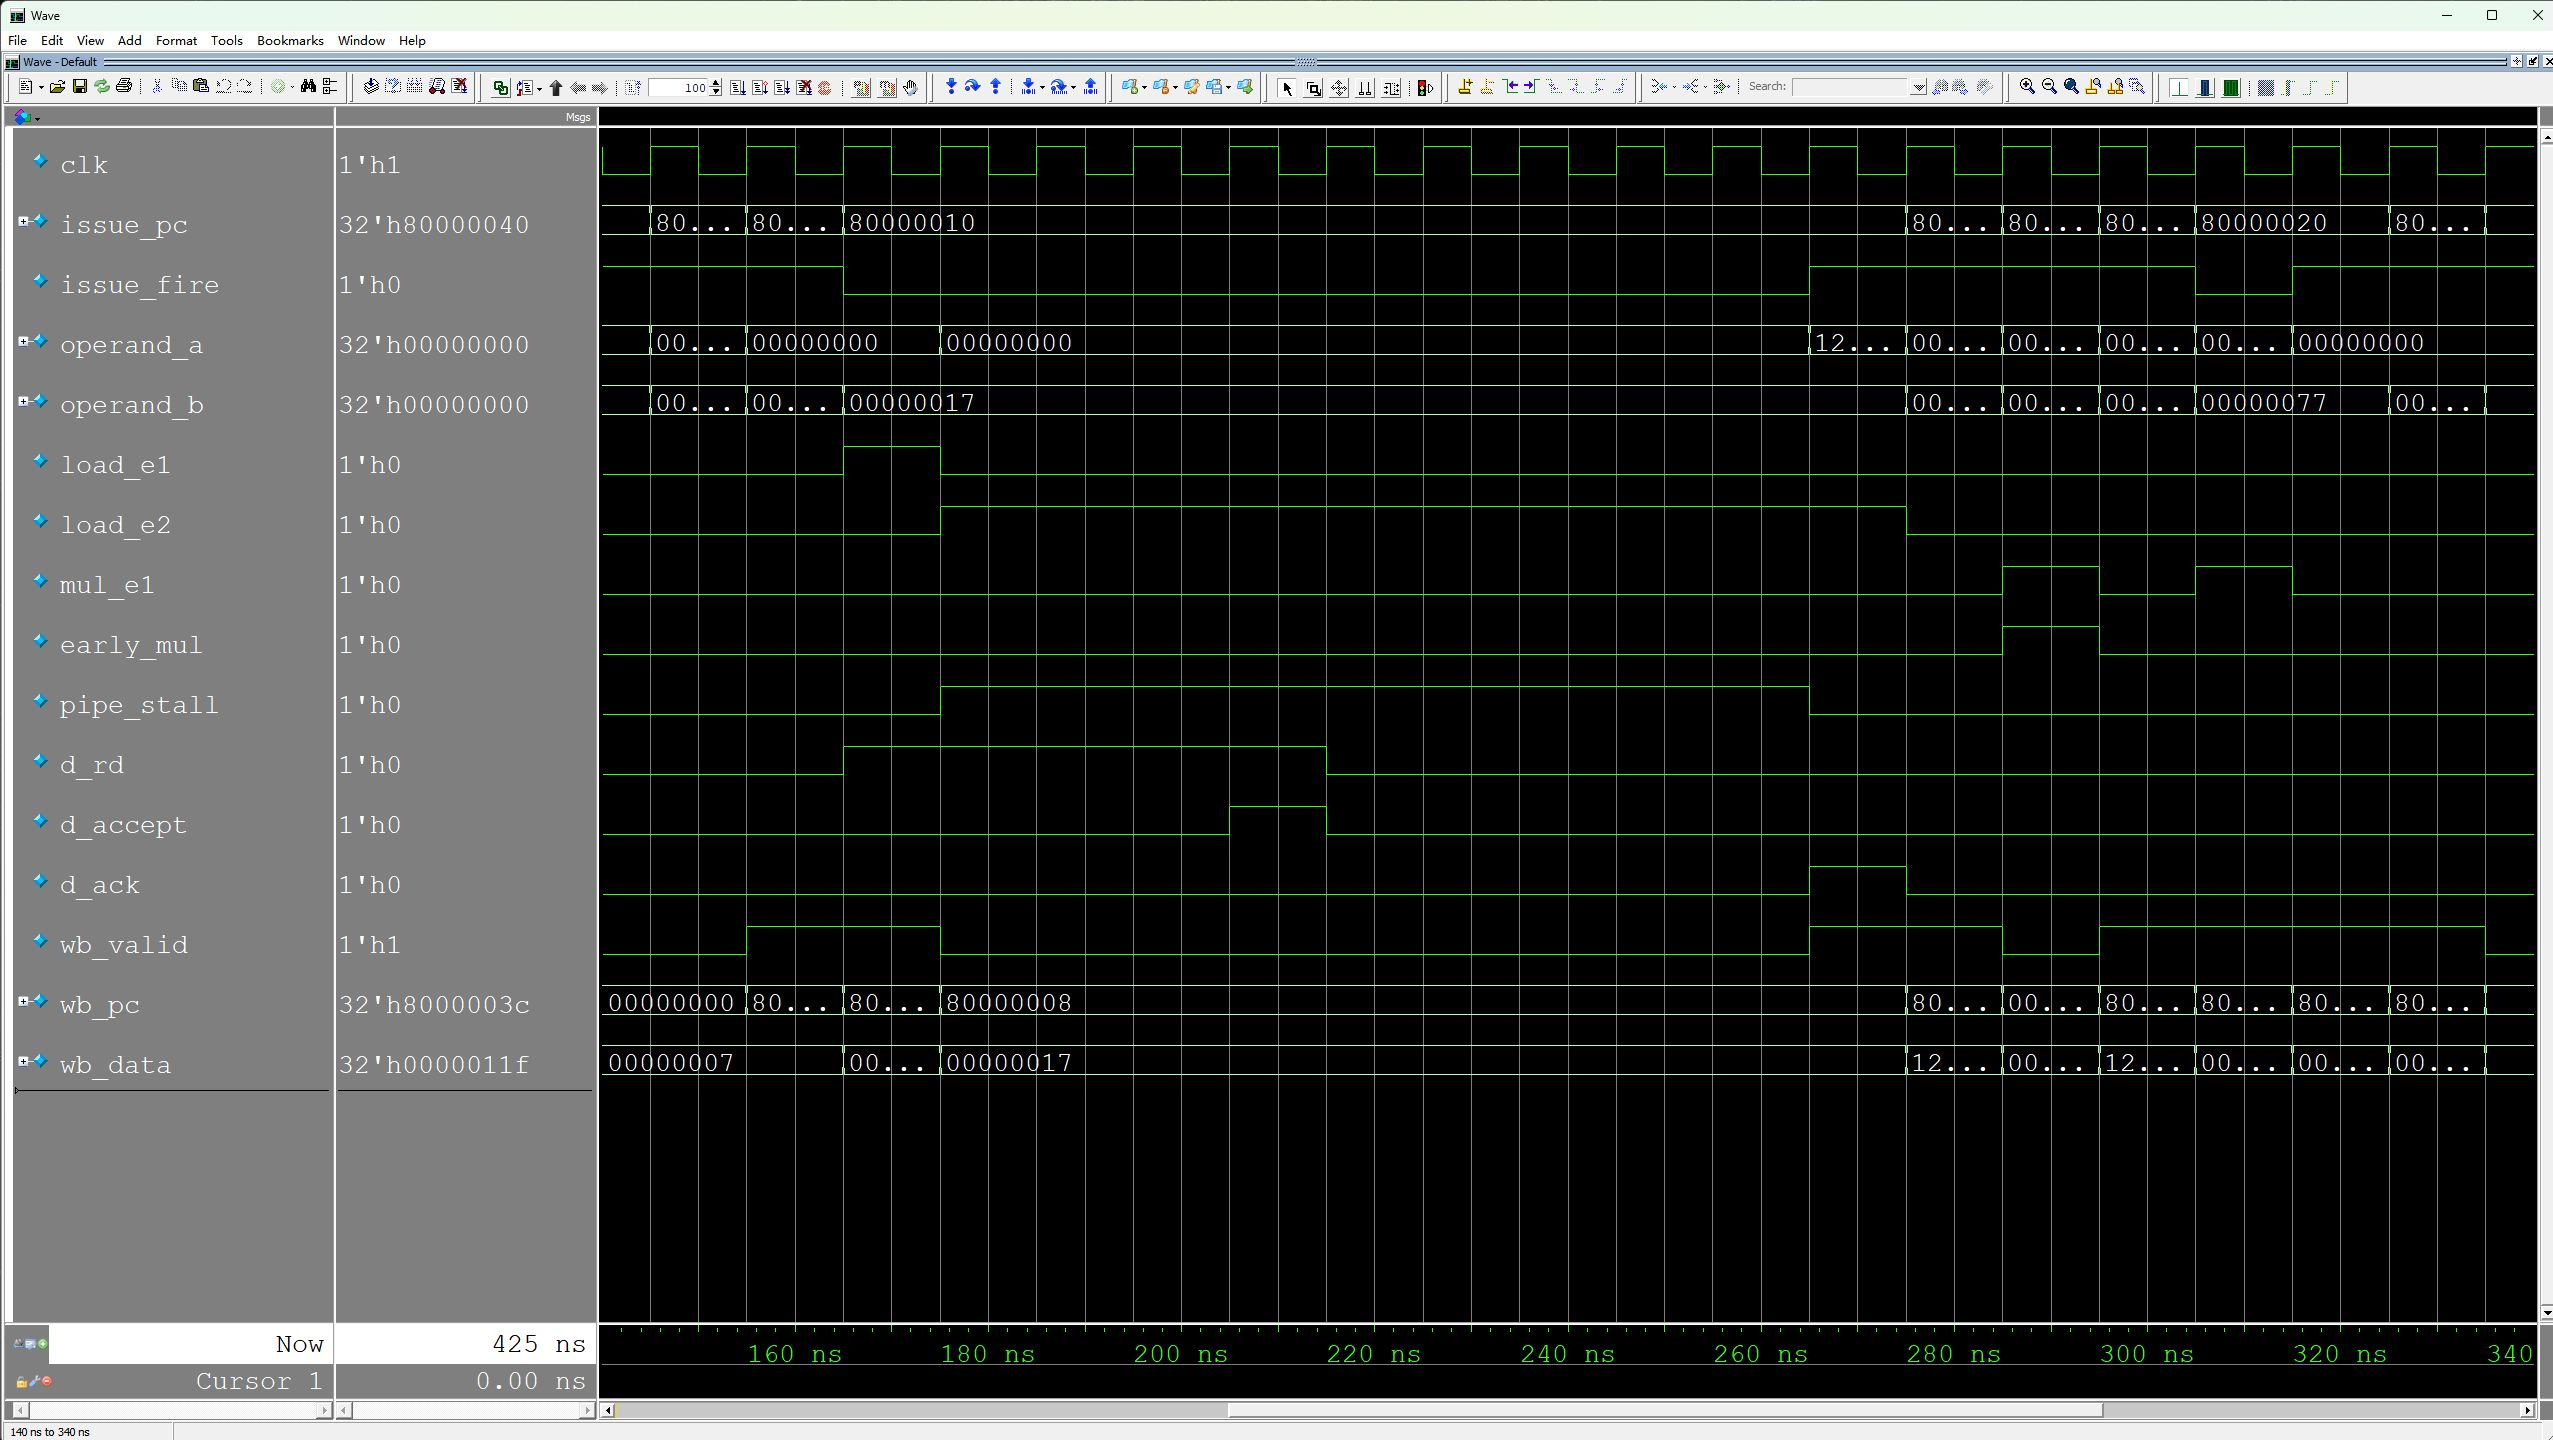
\includegraphics[width=0.8\linewidth]{../figure/cpu-module-issueflow-modelsim-original.jpg}
\caption{真实取指序列中的加载等待、乘法旁路和顺序写回波形}
\label{fig:cpu-module-issueflow}
\end{figure}

\subsubsection{LSU端口与异常响应}

LSU测试台连接公开的指令、操作数、请求和写回端口，按RISC-V访存规则给出预期数据、写掩码和异常编码。
测试覆盖字节、半字和字访问，覆盖未接纳时保持地址和写掩码、加载符号扩展、存储数据排列，以及非对齐和总线错误的精确响应。
18次访问中，11次加载和4次存储形成总线事务，其中2次返回总线错误；另有3次非对齐访问在发出总线请求前产生异常。
测试累计检查45个未接纳保持周期，完成220/220项检查。
图\ref{fig:cpu-module-lsu}依次给出字节、半字和字存储：写掩码为\texttt{8}、\texttt{C}和\texttt{F}，对应数据为\texttt{DD000000}、\texttt{CCDD0000}和\texttt{AABBCCDD}。
\texttt{accept}之前请求字段保持不变；后续非对齐访问仅产生\texttt{wb\_valid}，没有读写请求。

\begin{figure}[!htbp]
\centering
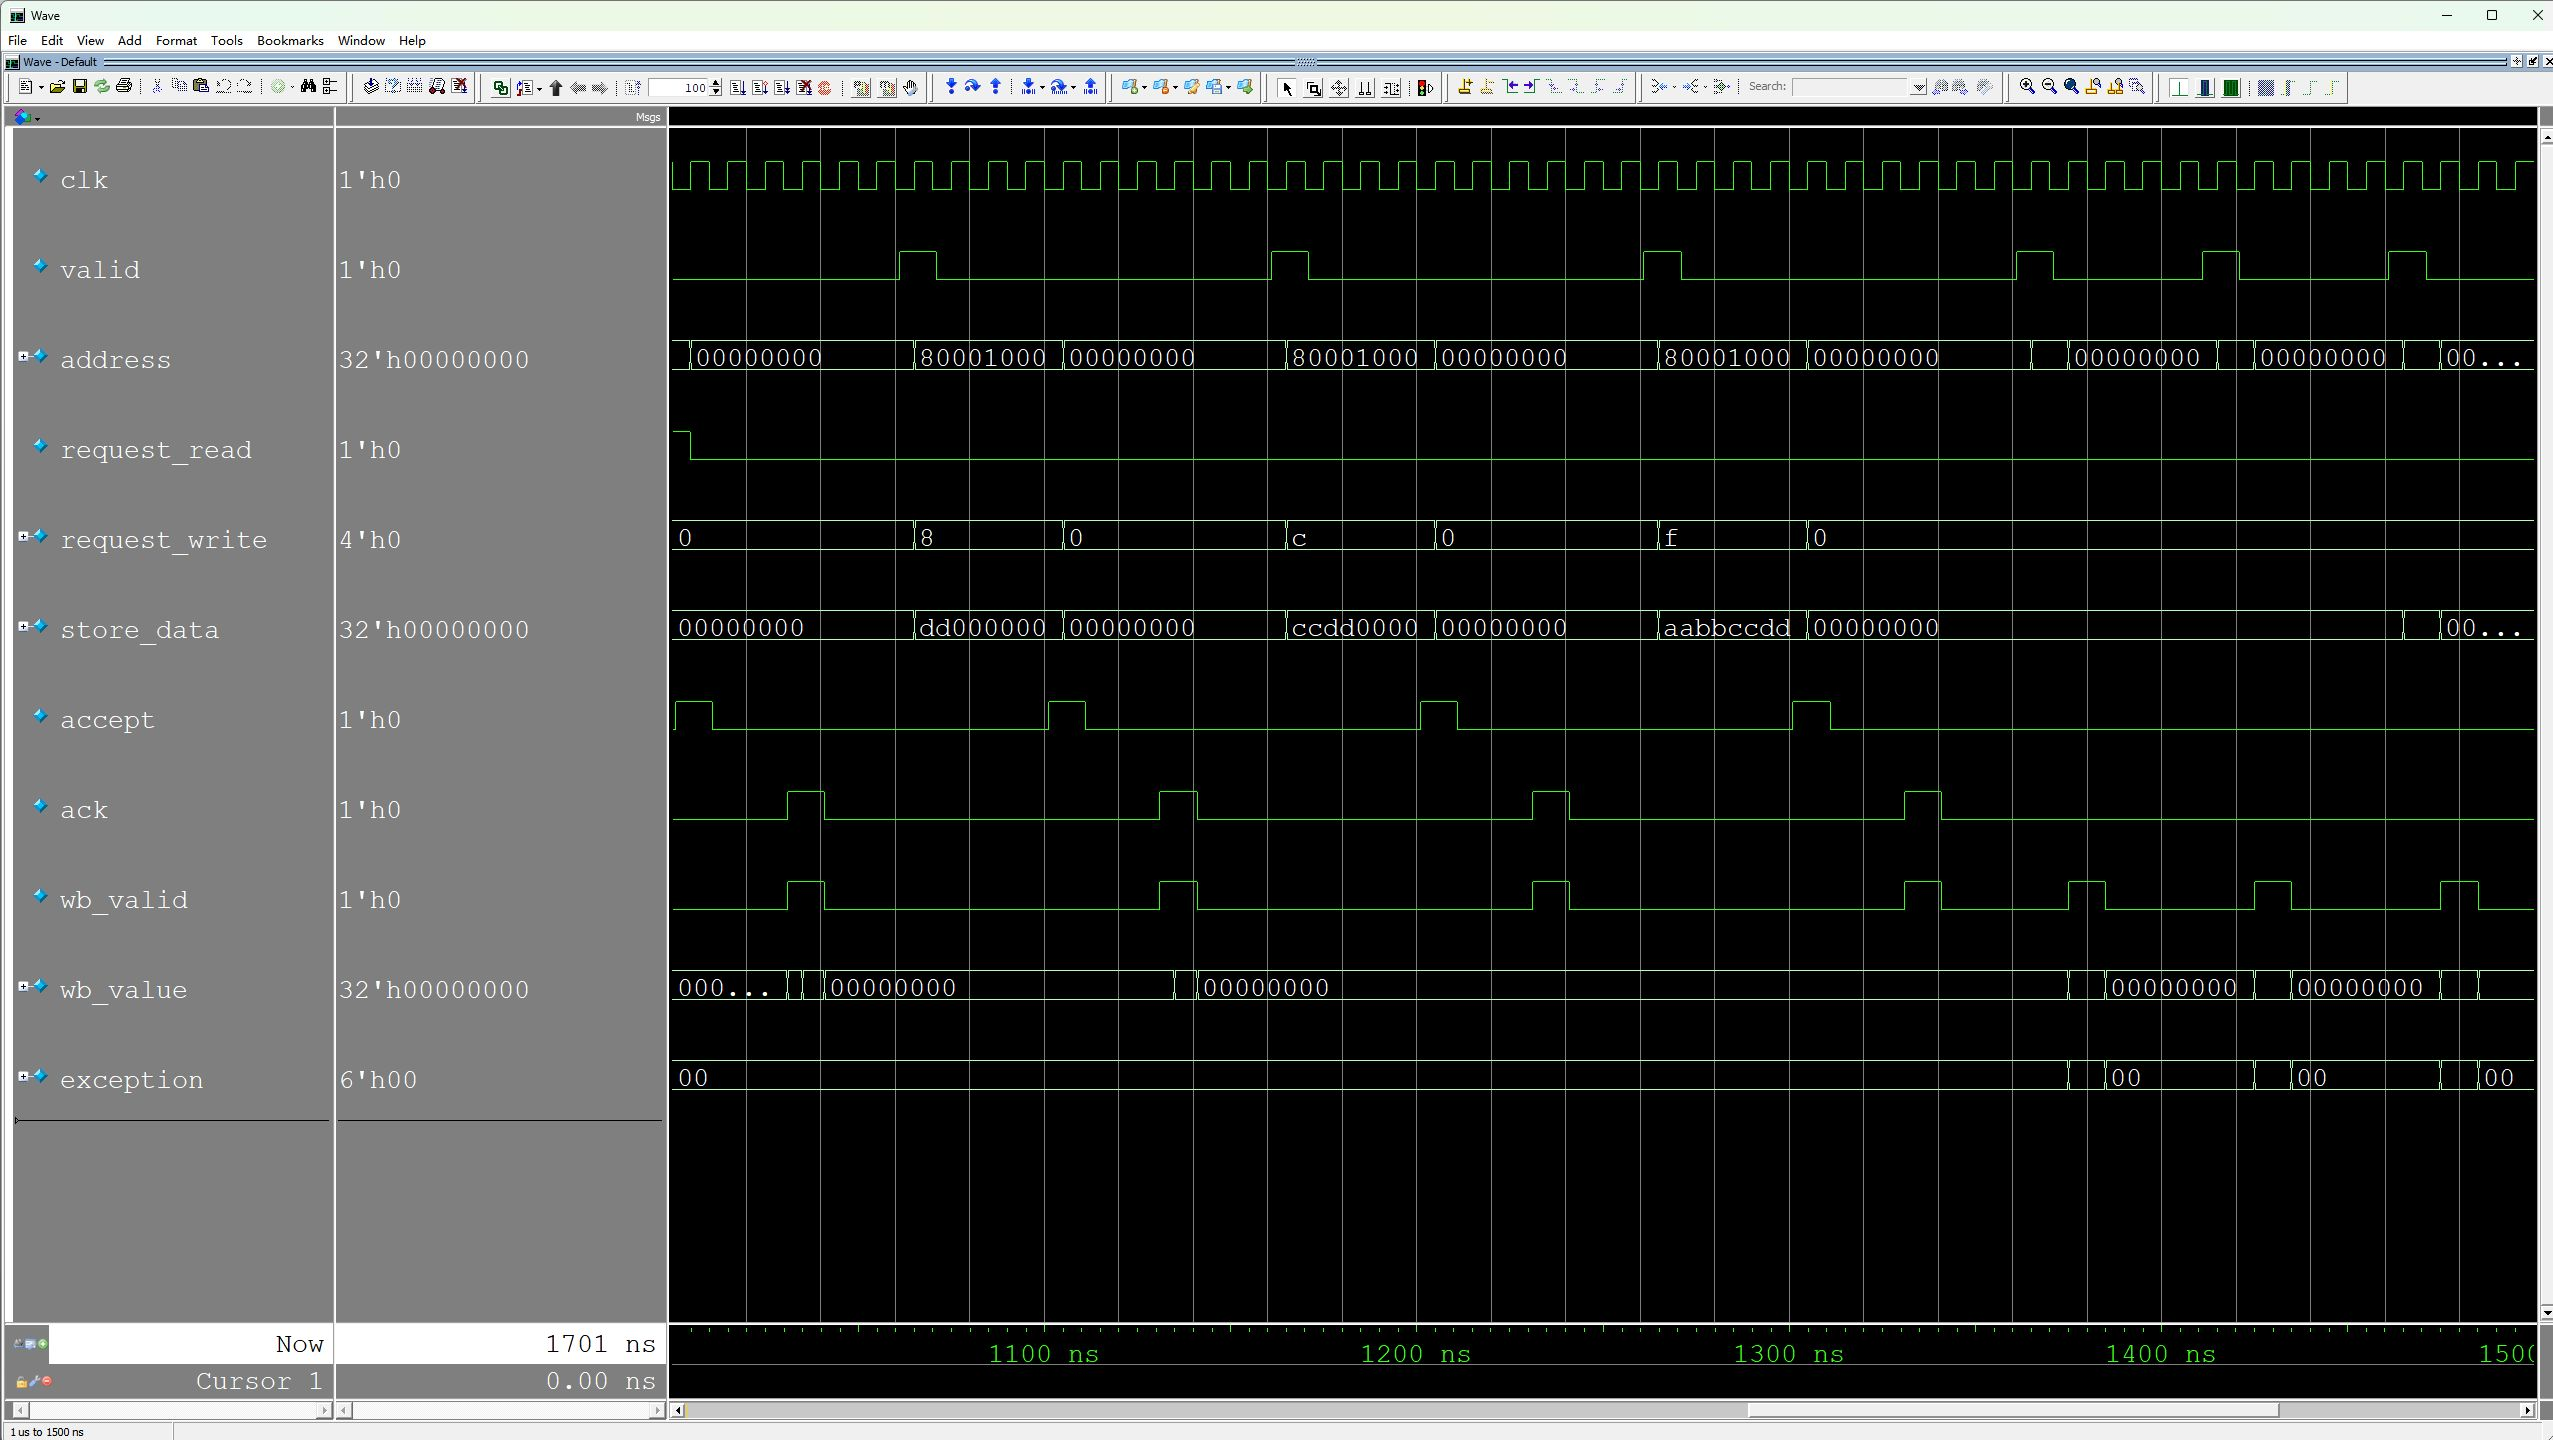
\includegraphics[width=0.8\linewidth]{../figure/cpu-module-lsu-modelsim-original.jpg}
\caption{LSU请求保持、字节写掩码和写回完成波形}
\label{fig:cpu-module-lsu}
\end{figure}

\subsubsection{I/D Cache命中、填充与维护}

Cache测试台使用独立的字节寻址内存模型，分别检查指令Cache填充和命中、数据Cache读写、行替换、写回、失效、刷新和错误重试。
组合测试完成1297/1297项检查，产生25次指令下层读、27次数据下层读和25次下层写，记录2次指令命中、2次数据命中及35个I/D同时在途周期。
图\ref{fig:cpu-module-icache}中，\texttt{arvalid}发起八拍填充，\texttt{rvalid}/\texttt{rlast}返回整行数据，第二次相同地址直接由\texttt{i\_valid}完成。

\begin{figure}[!htbp]
\centering
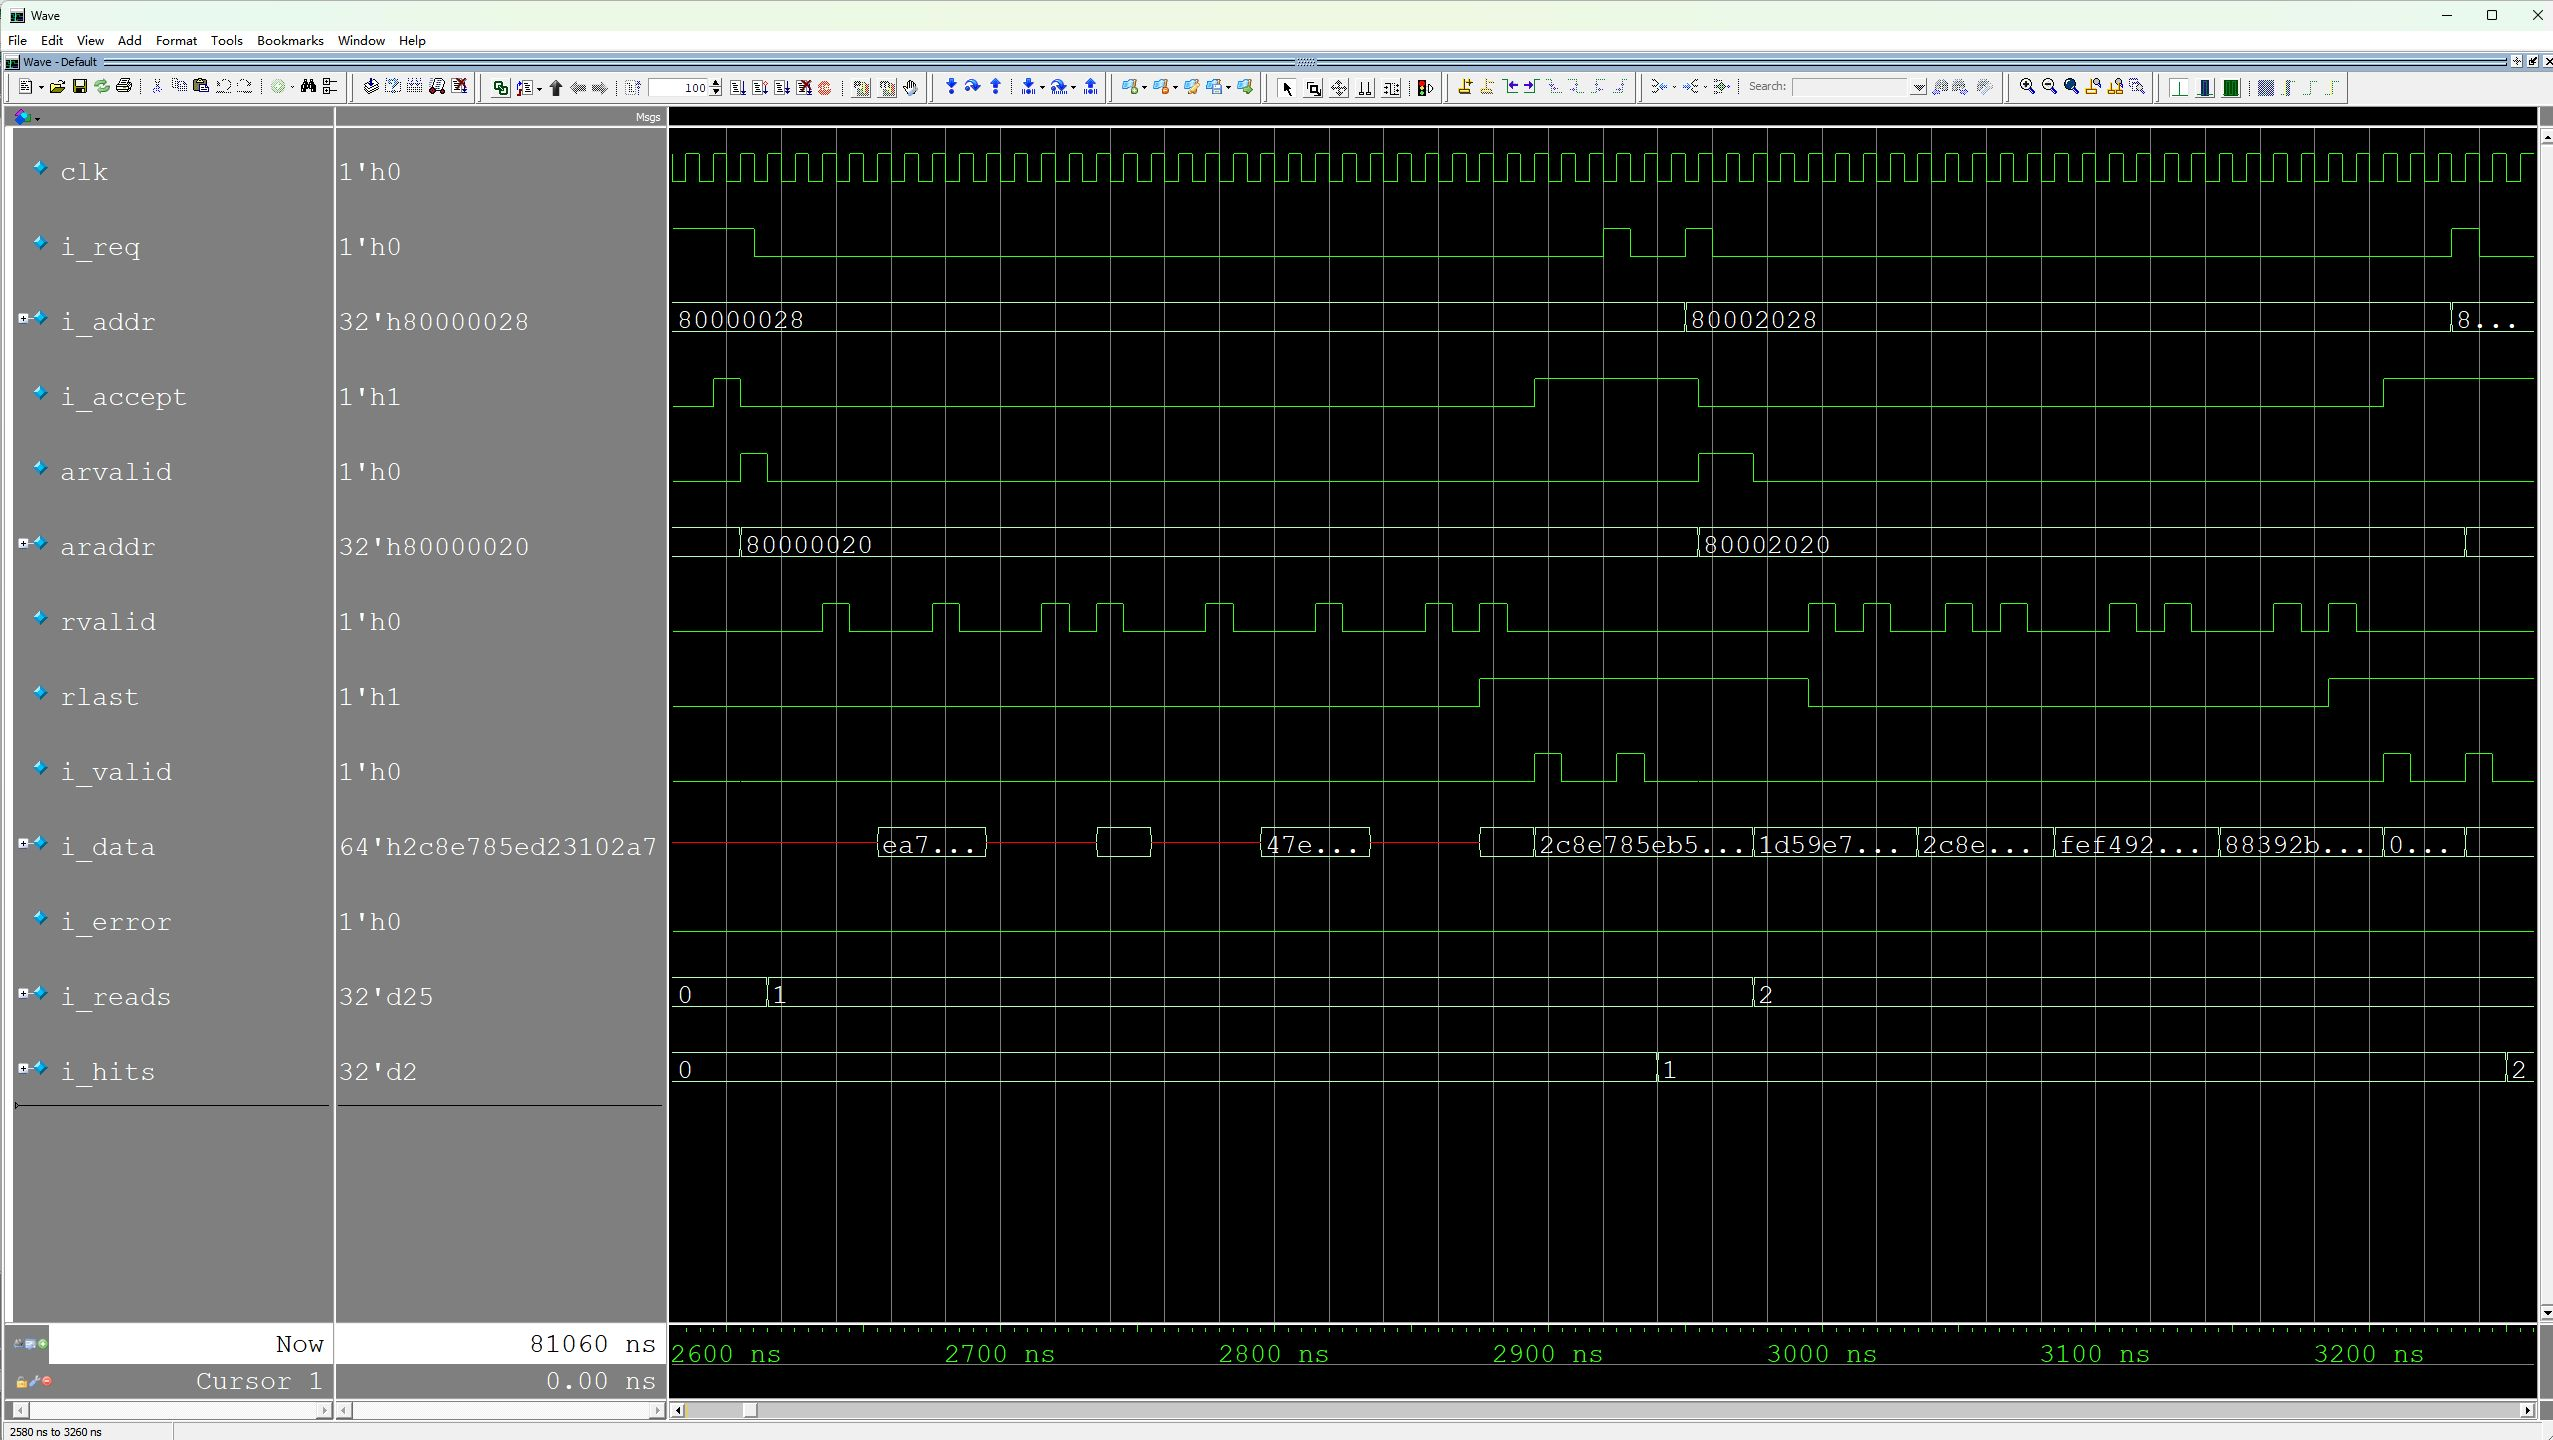
\includegraphics[width=0.8\linewidth]{../figure/cpu-module-icache-modelsim-original.jpg}
\caption{指令Cache填充、返回和命中波形}
\label{fig:cpu-module-icache}
\end{figure}

\subsubsection{数据Cache写回与维护}

写回测试完成1355/1355项检查、35次下层读和184次下层写，覆盖全部15种非零字节掩码、脏行清理、替换前写回、整Cache刷新和共享区旁路。
测试逐一在八个写回字上注入下层错误，检查失败后仍能读取脏数据，重新清理时完整写回八个字；填充错误也逐拍注入，失败行不得变为有效行。
图\ref{fig:cpu-module-dcache-writeback}中，\texttt{clean}启动行清理，\texttt{writes}由0递增至8，\texttt{ack}在最后一次下层写响应后给出；随后再次读取和清理没有新增下层读写。

\begin{figure}[!htbp]
\centering
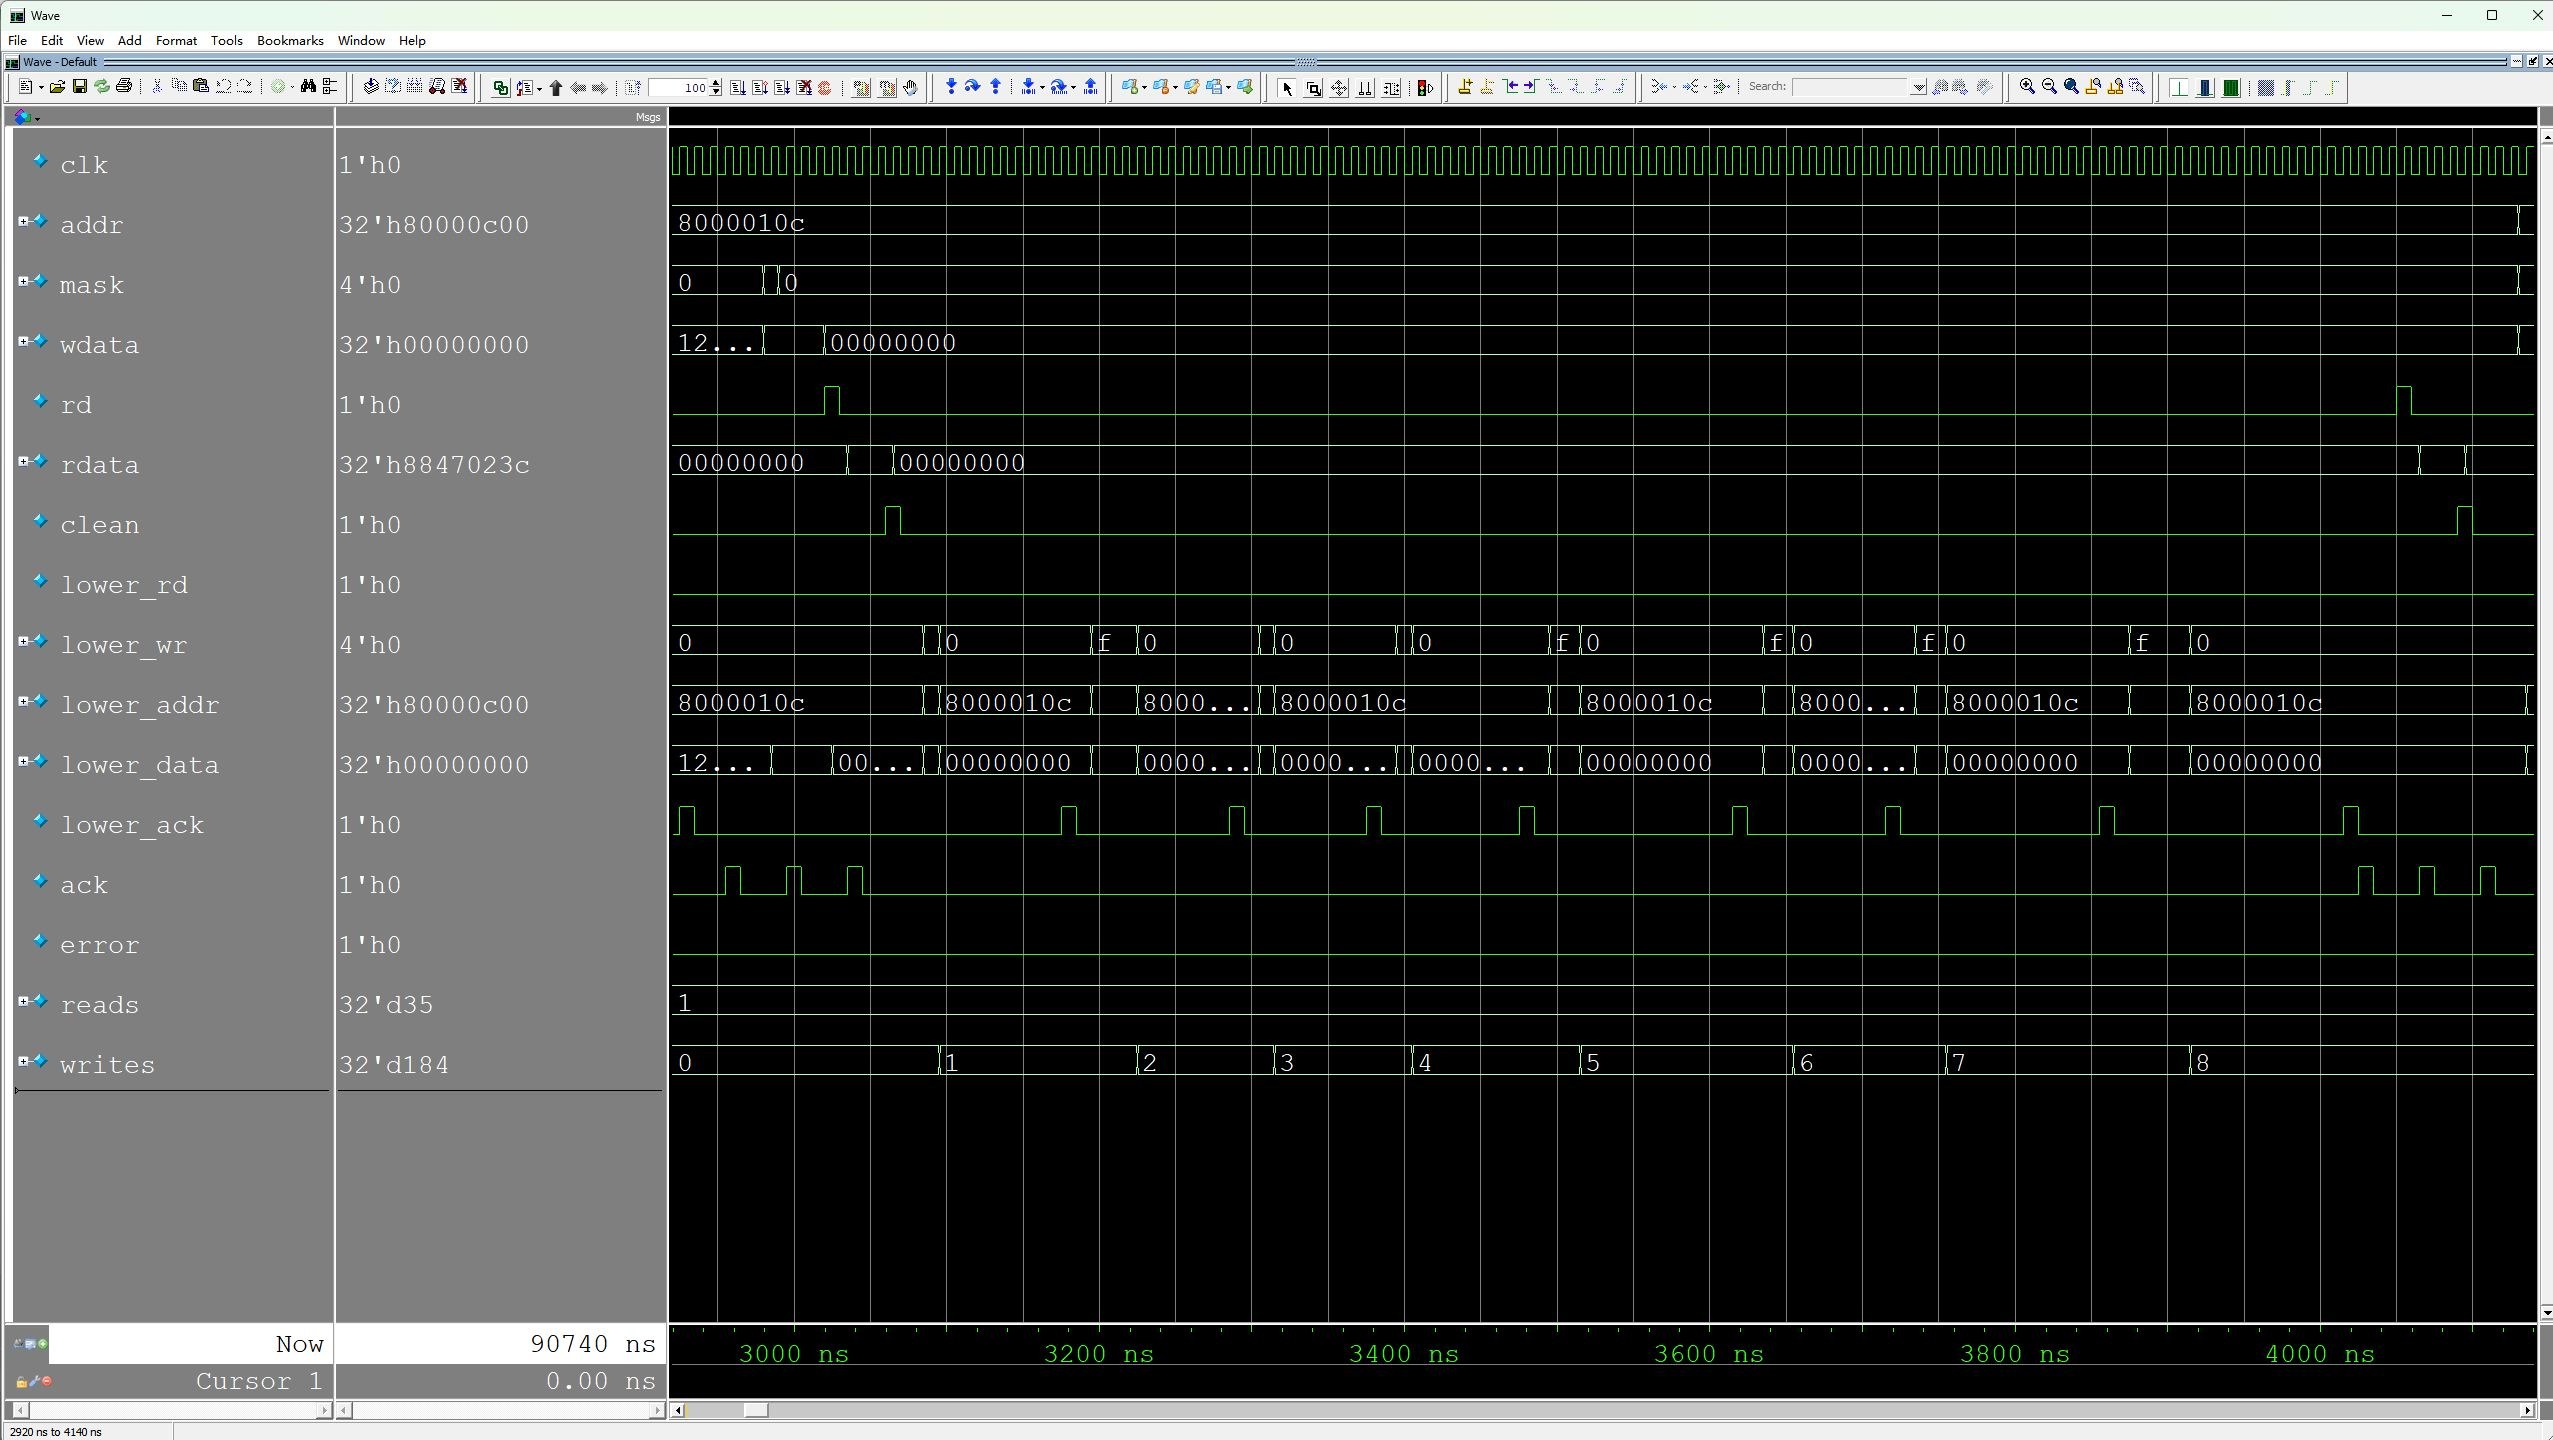
\includegraphics[width=0.8\linewidth]{../figure/cpu-module-dcache-writeback-modelsim-original.jpg}
\caption{数据Cache脏行写回和清理完成波形}
\label{fig:cpu-module-dcache-writeback}
\end{figure}

\subsubsection{数据Cache响应重叠}

重叠测试完成142/142项检查、11次下层读和25次下层写，覆盖命中读取响应与下一请求重叠、标签顺序、跨组跨标记访问和错误响应隔离。
图\ref{fig:cpu-module-dcache-overlap}在\texttt{score\_active}期间连续发出12次命中读取，\texttt{tail}统计接纳数、\texttt{head}统计返回数，最终均为12。
命中读取每两个时钟周期接纳一次，\texttt{accept}与旧请求\texttt{ack}在完成边沿重叠，\texttt{resp\_tag}按顺序返回，期间\texttt{lower\_rd}保持为零。
测试还分别接入存储、Cache维护、共享区读取及下层错误，检查返回错误响应时不接纳后续请求、存储更新保持串行，脏行替换失败后数据仍可读取。

\begin{figure}[!htbp]
\centering
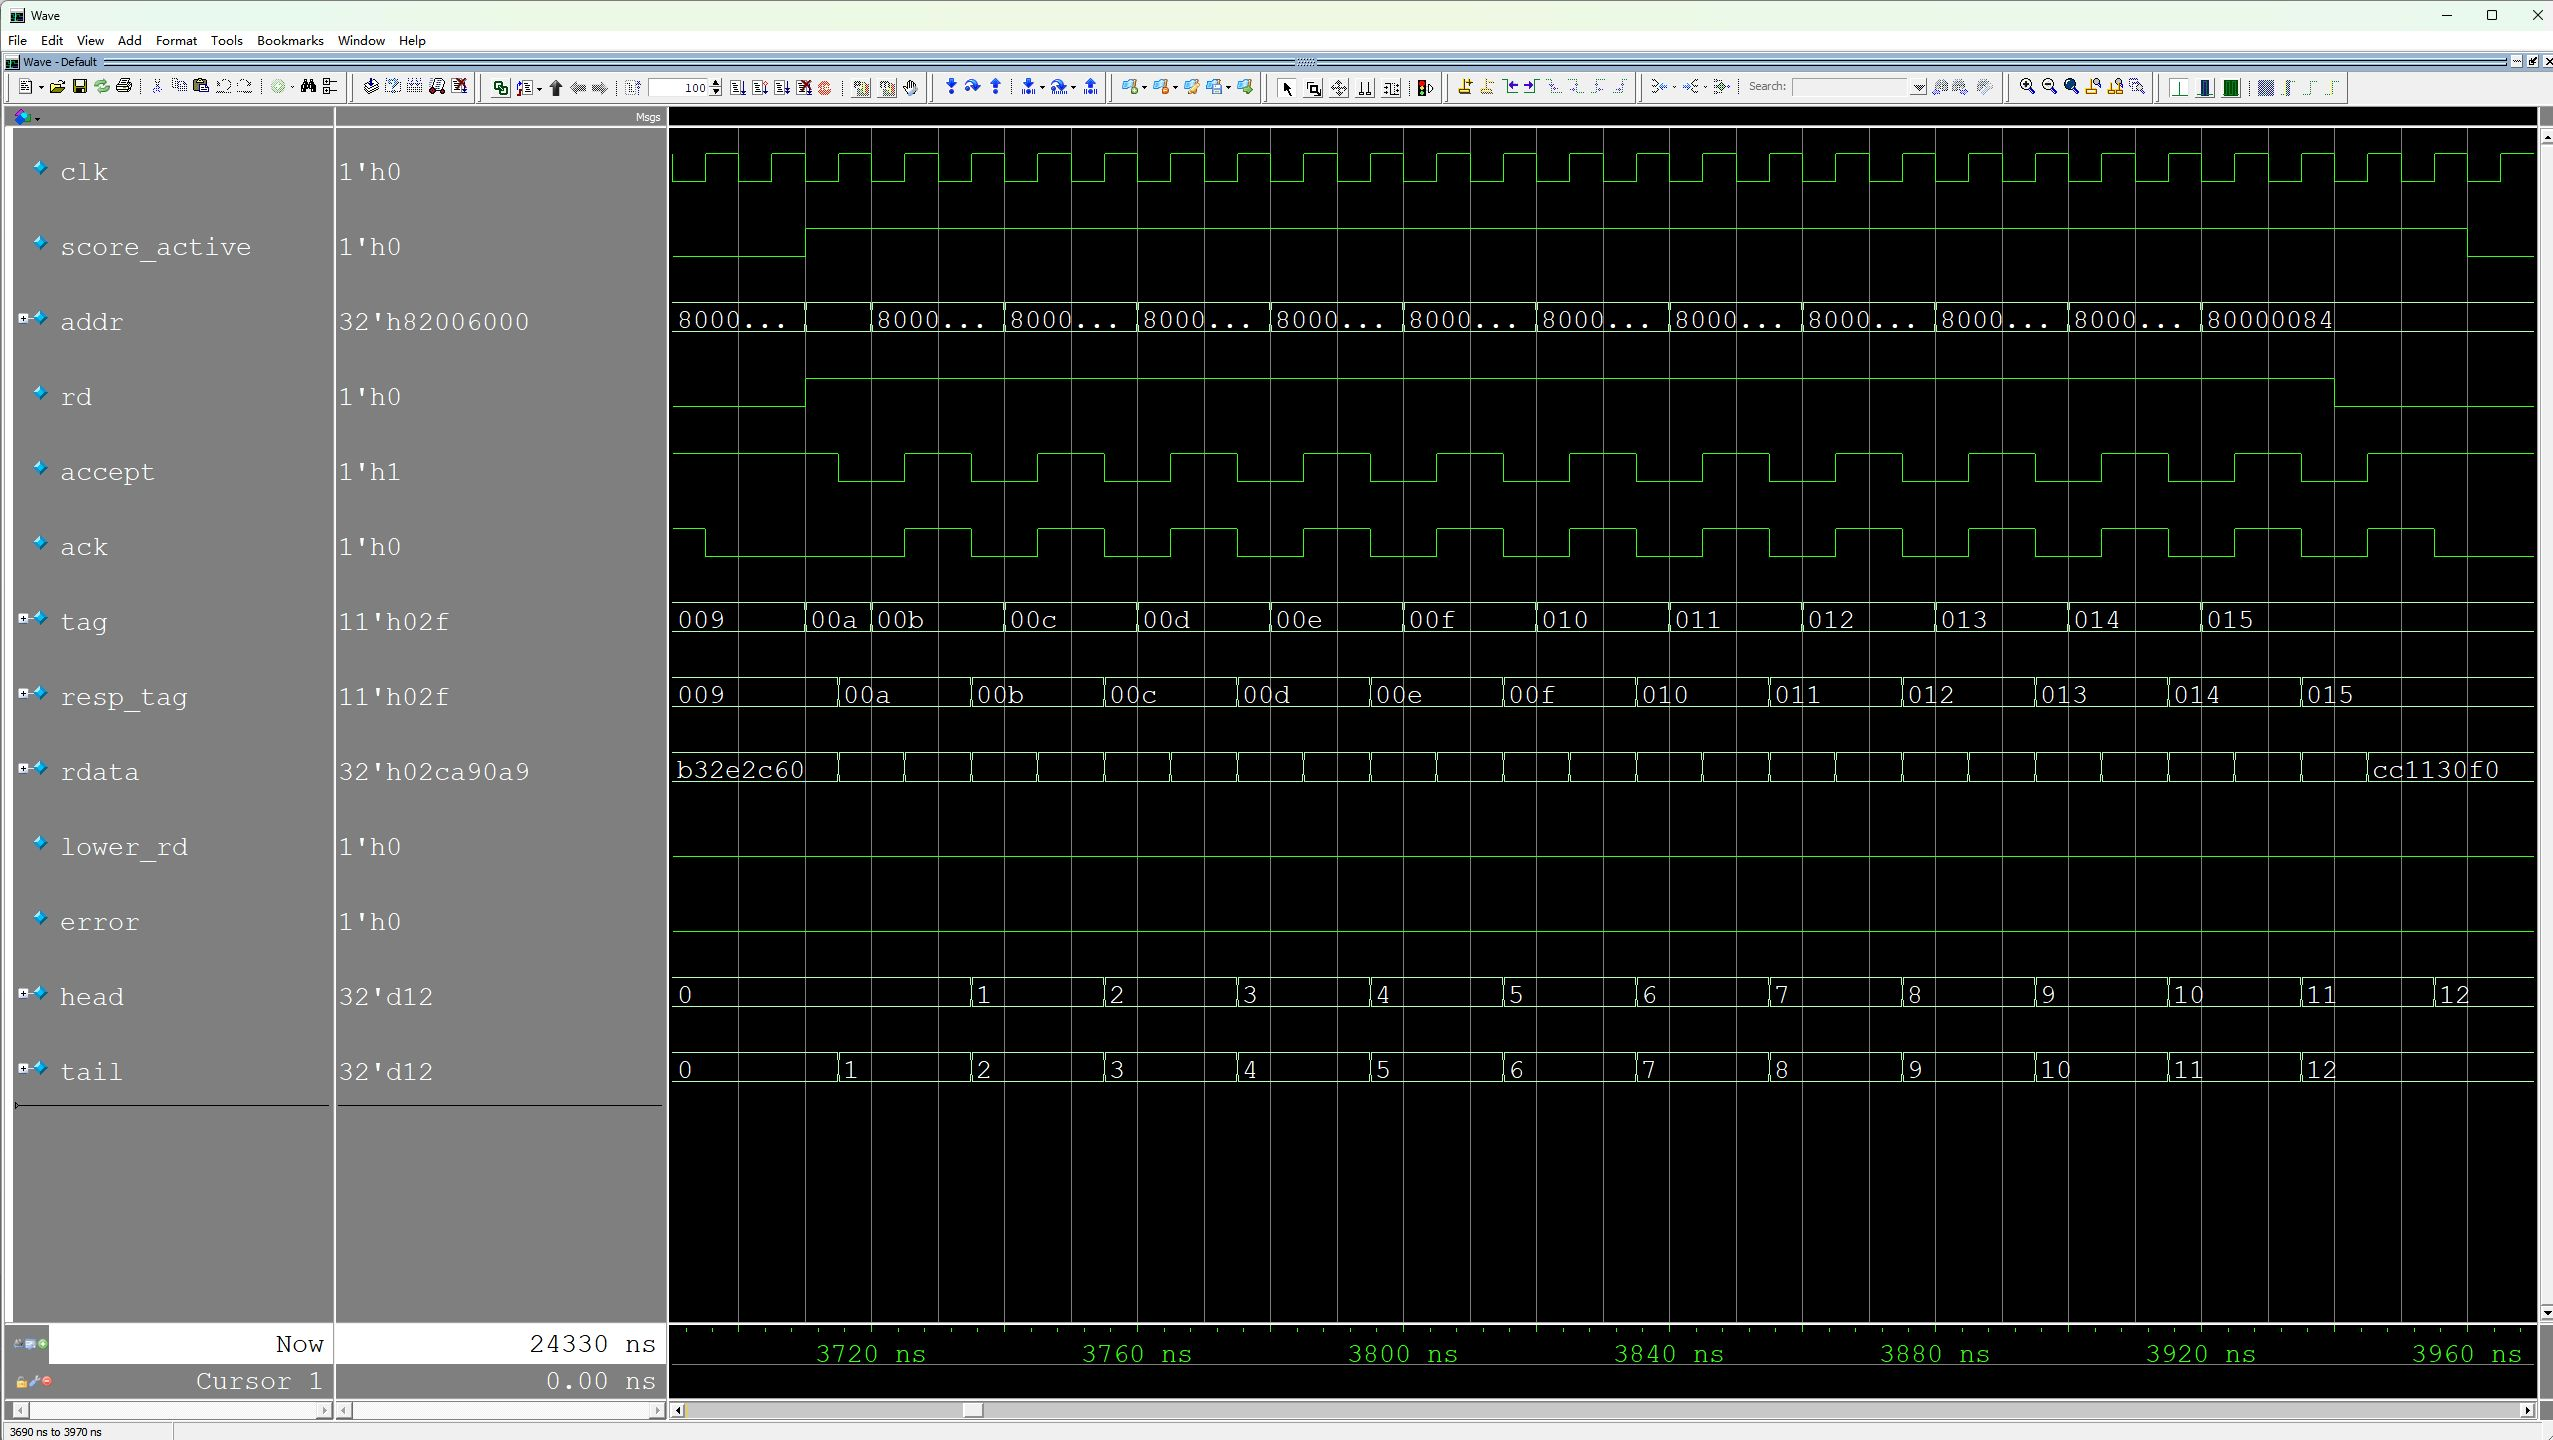
\includegraphics[width=0.8\linewidth]{../figure/cpu-module-dcache-overlap-modelsim-original.jpg}
\caption{数据Cache响应重叠、标签顺序和连续命中波形}
\label{fig:cpu-module-dcache-overlap}
\end{figure}

\subsection{系统级仿真验证}

\subsubsection{存储访问与故障处理}

系统级测试使用最小固件连接Boot ROM、片上SRAM、UART、私有Cache、共享区旁路和模型AXI128下层。
缓存配置下完成启动、私有区读写、共享区读写、\texttt{FENCE.I}后的代码执行、DDR就绪等待、下层读错误和平台故障后的本地访问；固件通过\texttt{mtvec}/\texttt{mepc}/\texttt{mcause}/\texttt{mtval}检查三次受控异常返回。
正例自检完成1277项检查，统计26356个时钟周期、14次读事务、35次写事务和3次陷阱，返回码为零。
图\ref{fig:cpu-system-cache-runtime}选取第三次异常：平台故障使\texttt{ddr\_ready}撤销、\texttt{fault}锁存；随后访存错误使\texttt{trap\_count}从2变为3，\texttt{mcause}=5、\texttt{mtval}=\texttt{0x80000000}。
异常处理程序将\texttt{mepc}从\texttt{0x000101FC}加4至\texttt{0x00010200}后执行\texttt{MRET}；程序继续访问片上存储，最终\texttt{done}=1且\texttt{exit\_code}=0。

\begin{figure}[!htbp]
\centering
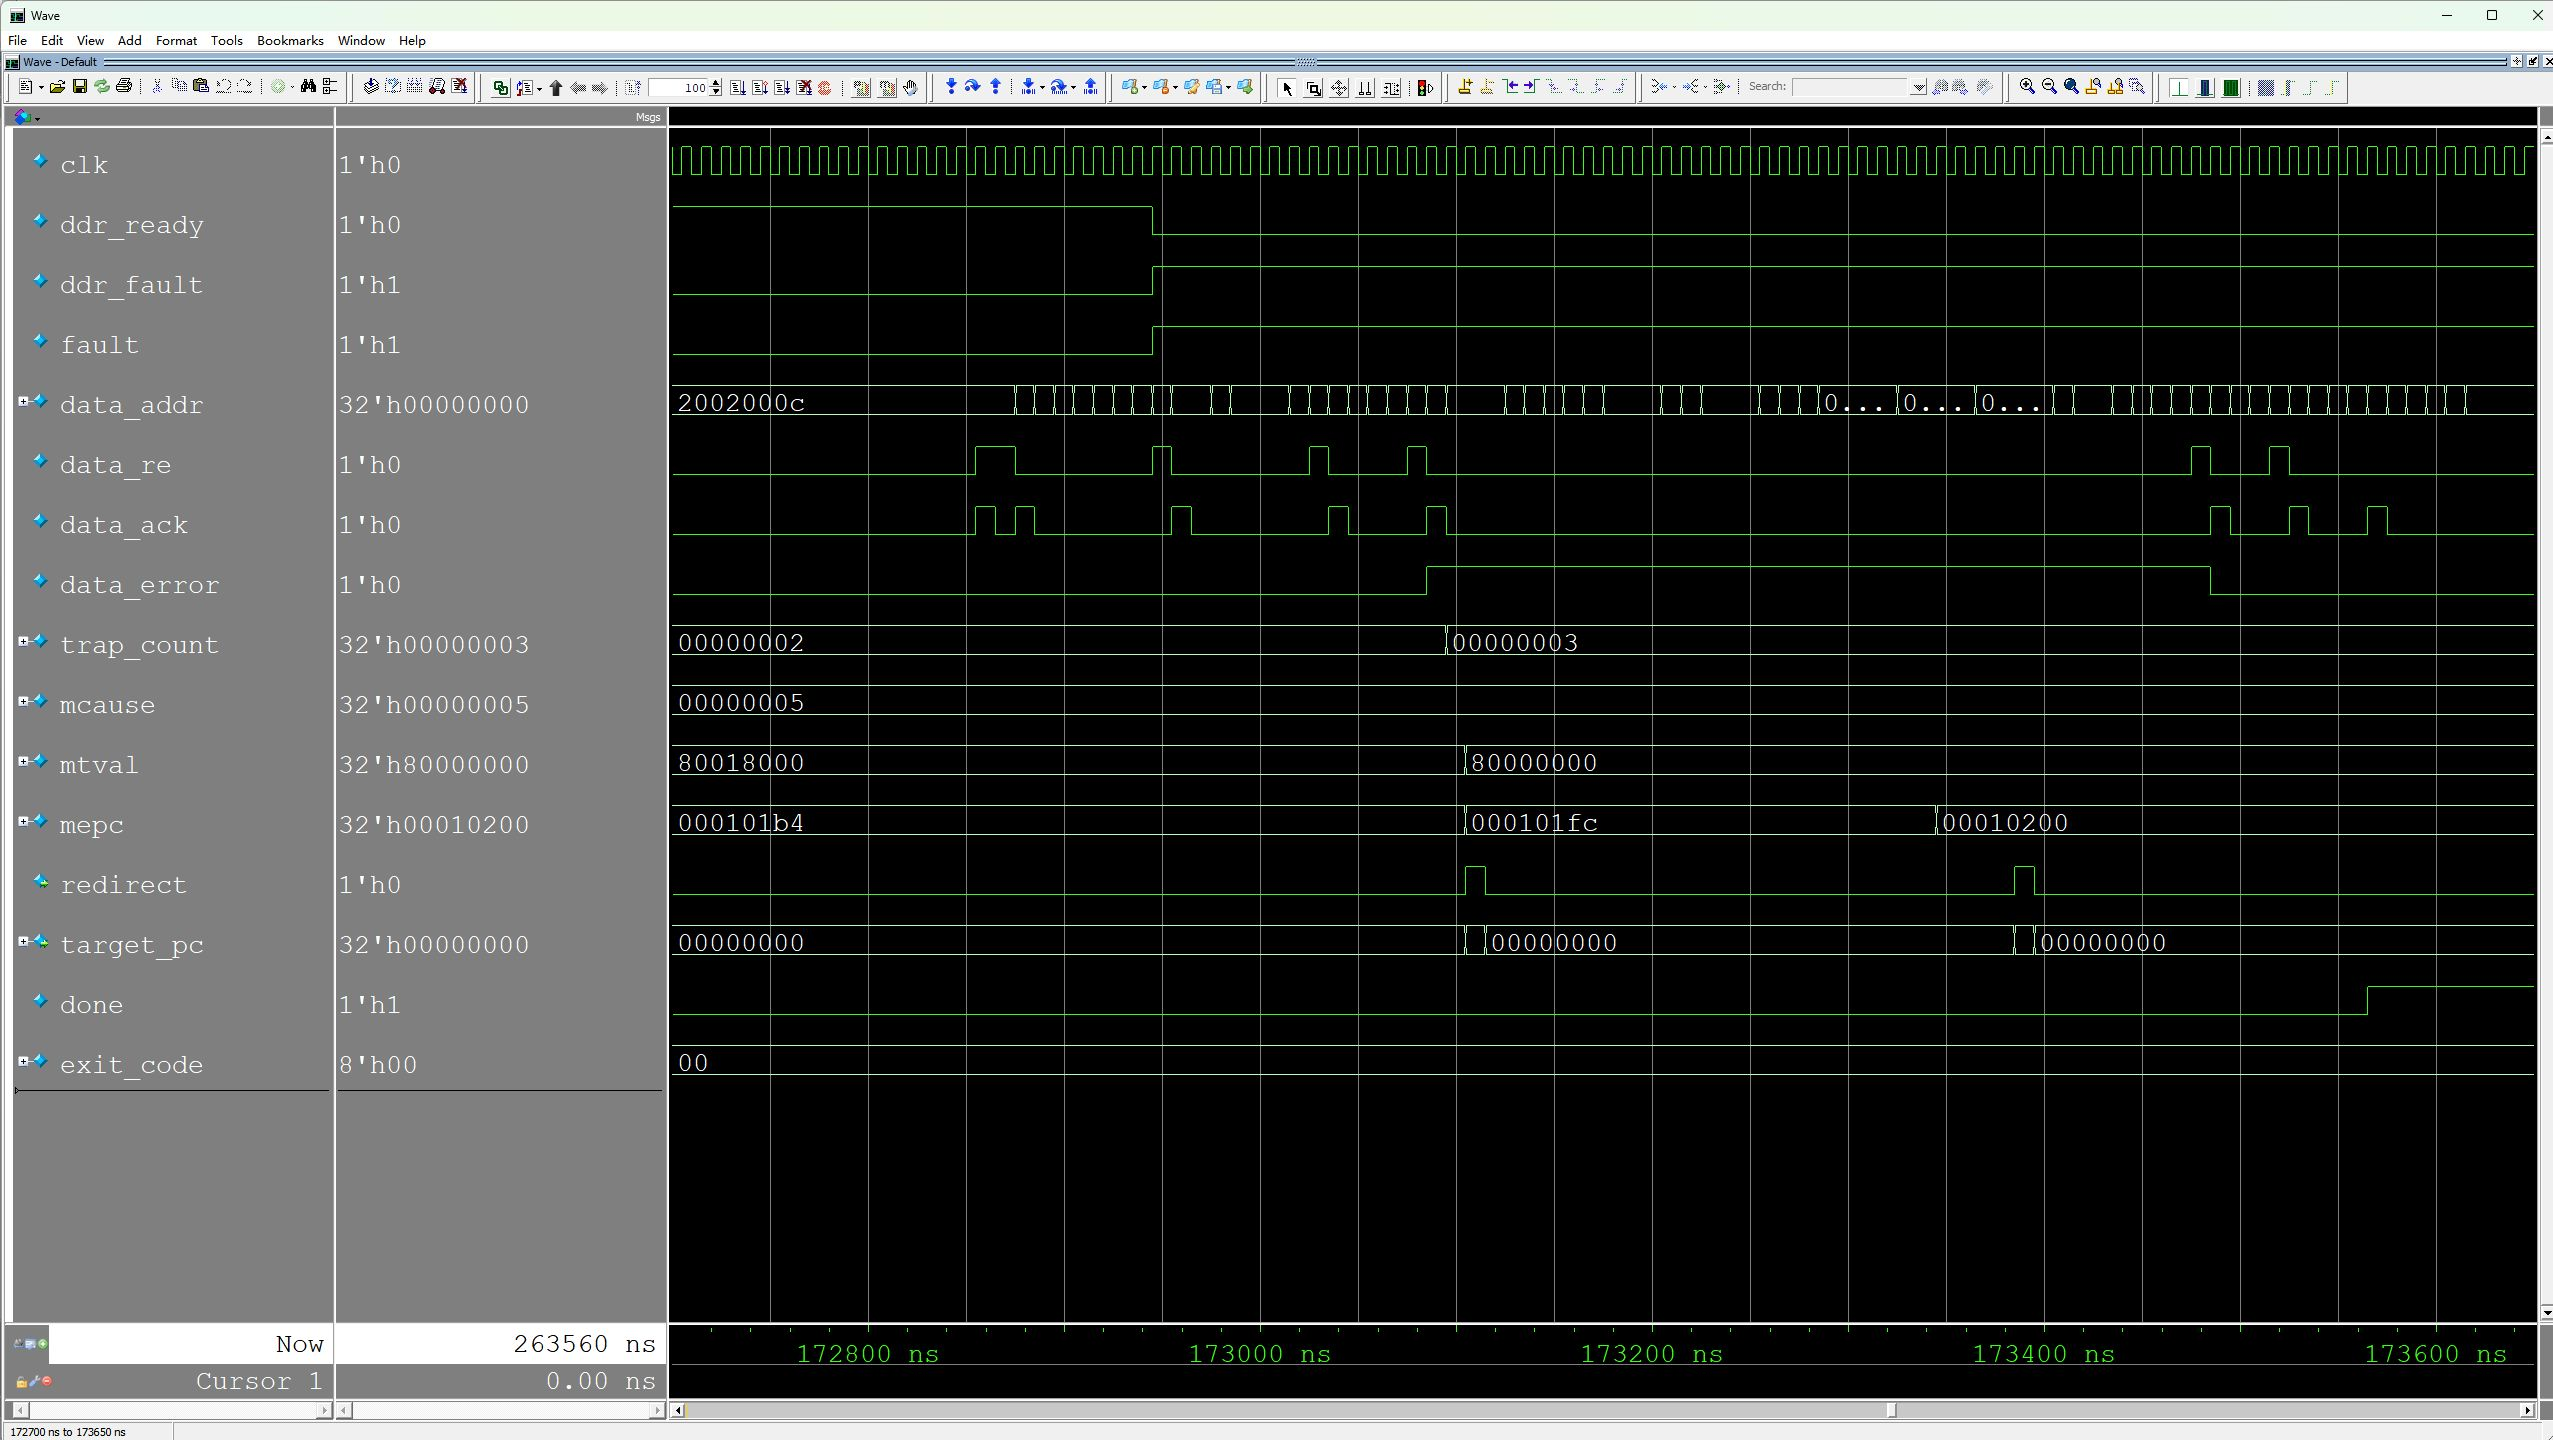
\includegraphics[width=0.8\linewidth]{../figure/cpu-system-cache-runtime-modelsim-original.jpg}
\caption{整核固件的平台故障、访存异常与MRET返回波形}
\label{fig:cpu-system-cache-runtime}
\end{figure}

独立路由测试完成476项检查、12次读事务和9次写事务，覆盖片上地址不出DDR、DDR未就绪时请求保持、I/D命中与共享区旁路、部分写掩码、响应所有权、错误锁存及复位恢复。
同一固件关闭Cache后通过809项检查，作为存储属性对照。下层读数据异或一位的错误注入在固件退出检查处触发失败，负例退出码为1。
原始日志、固件、WLF/VCD与截图保存在\path{docs/verification/cpu/system_support/}。
上述结果来自ModelSim中使用行为级AXI内存模型的数字仿真。

\subsubsection{外部中断进入与返回}

中断测试采用单发射核、512项直接映射BTB、512项BHT和4项RAS，关闭GShare，连接128\,KiB行为级指令与数据存储器。
固件先检查8类同步异常，再设置\texttt{mie.MEIE}和\texttt{mstatus.MIE}；测试台在触发地址的存储请求被接纳后驱动外部\texttt{irq}。
中断处理程序检查机器外部中断原因，清除\texttt{mie}、将处理计数加一，再执行\texttt{MRET}；返回后固件检查计数恰好为一并正常退出。

图\ref{fig:cpu-system-external-irq}中，中断进入时\texttt{mcause}=\texttt{0x8000000B}，\texttt{mepc}=\texttt{0x80000150}，\texttt{mtval}=0。
\texttt{mstatus}由\texttt{0x00000088}变为\texttt{0x00001880}，对应MIE清零、MPIE置位和机器态保存；\texttt{MRET}后恢复为\texttt{0x00000088}，退休记录从保存的\texttt{mepc}继续执行。
固件完成3582个周期、864次退休和92次存储，8类同步异常与1次外部中断的覆盖掩码为\texttt{0x1FF}。

\begin{figure}[!htbp]
\centering
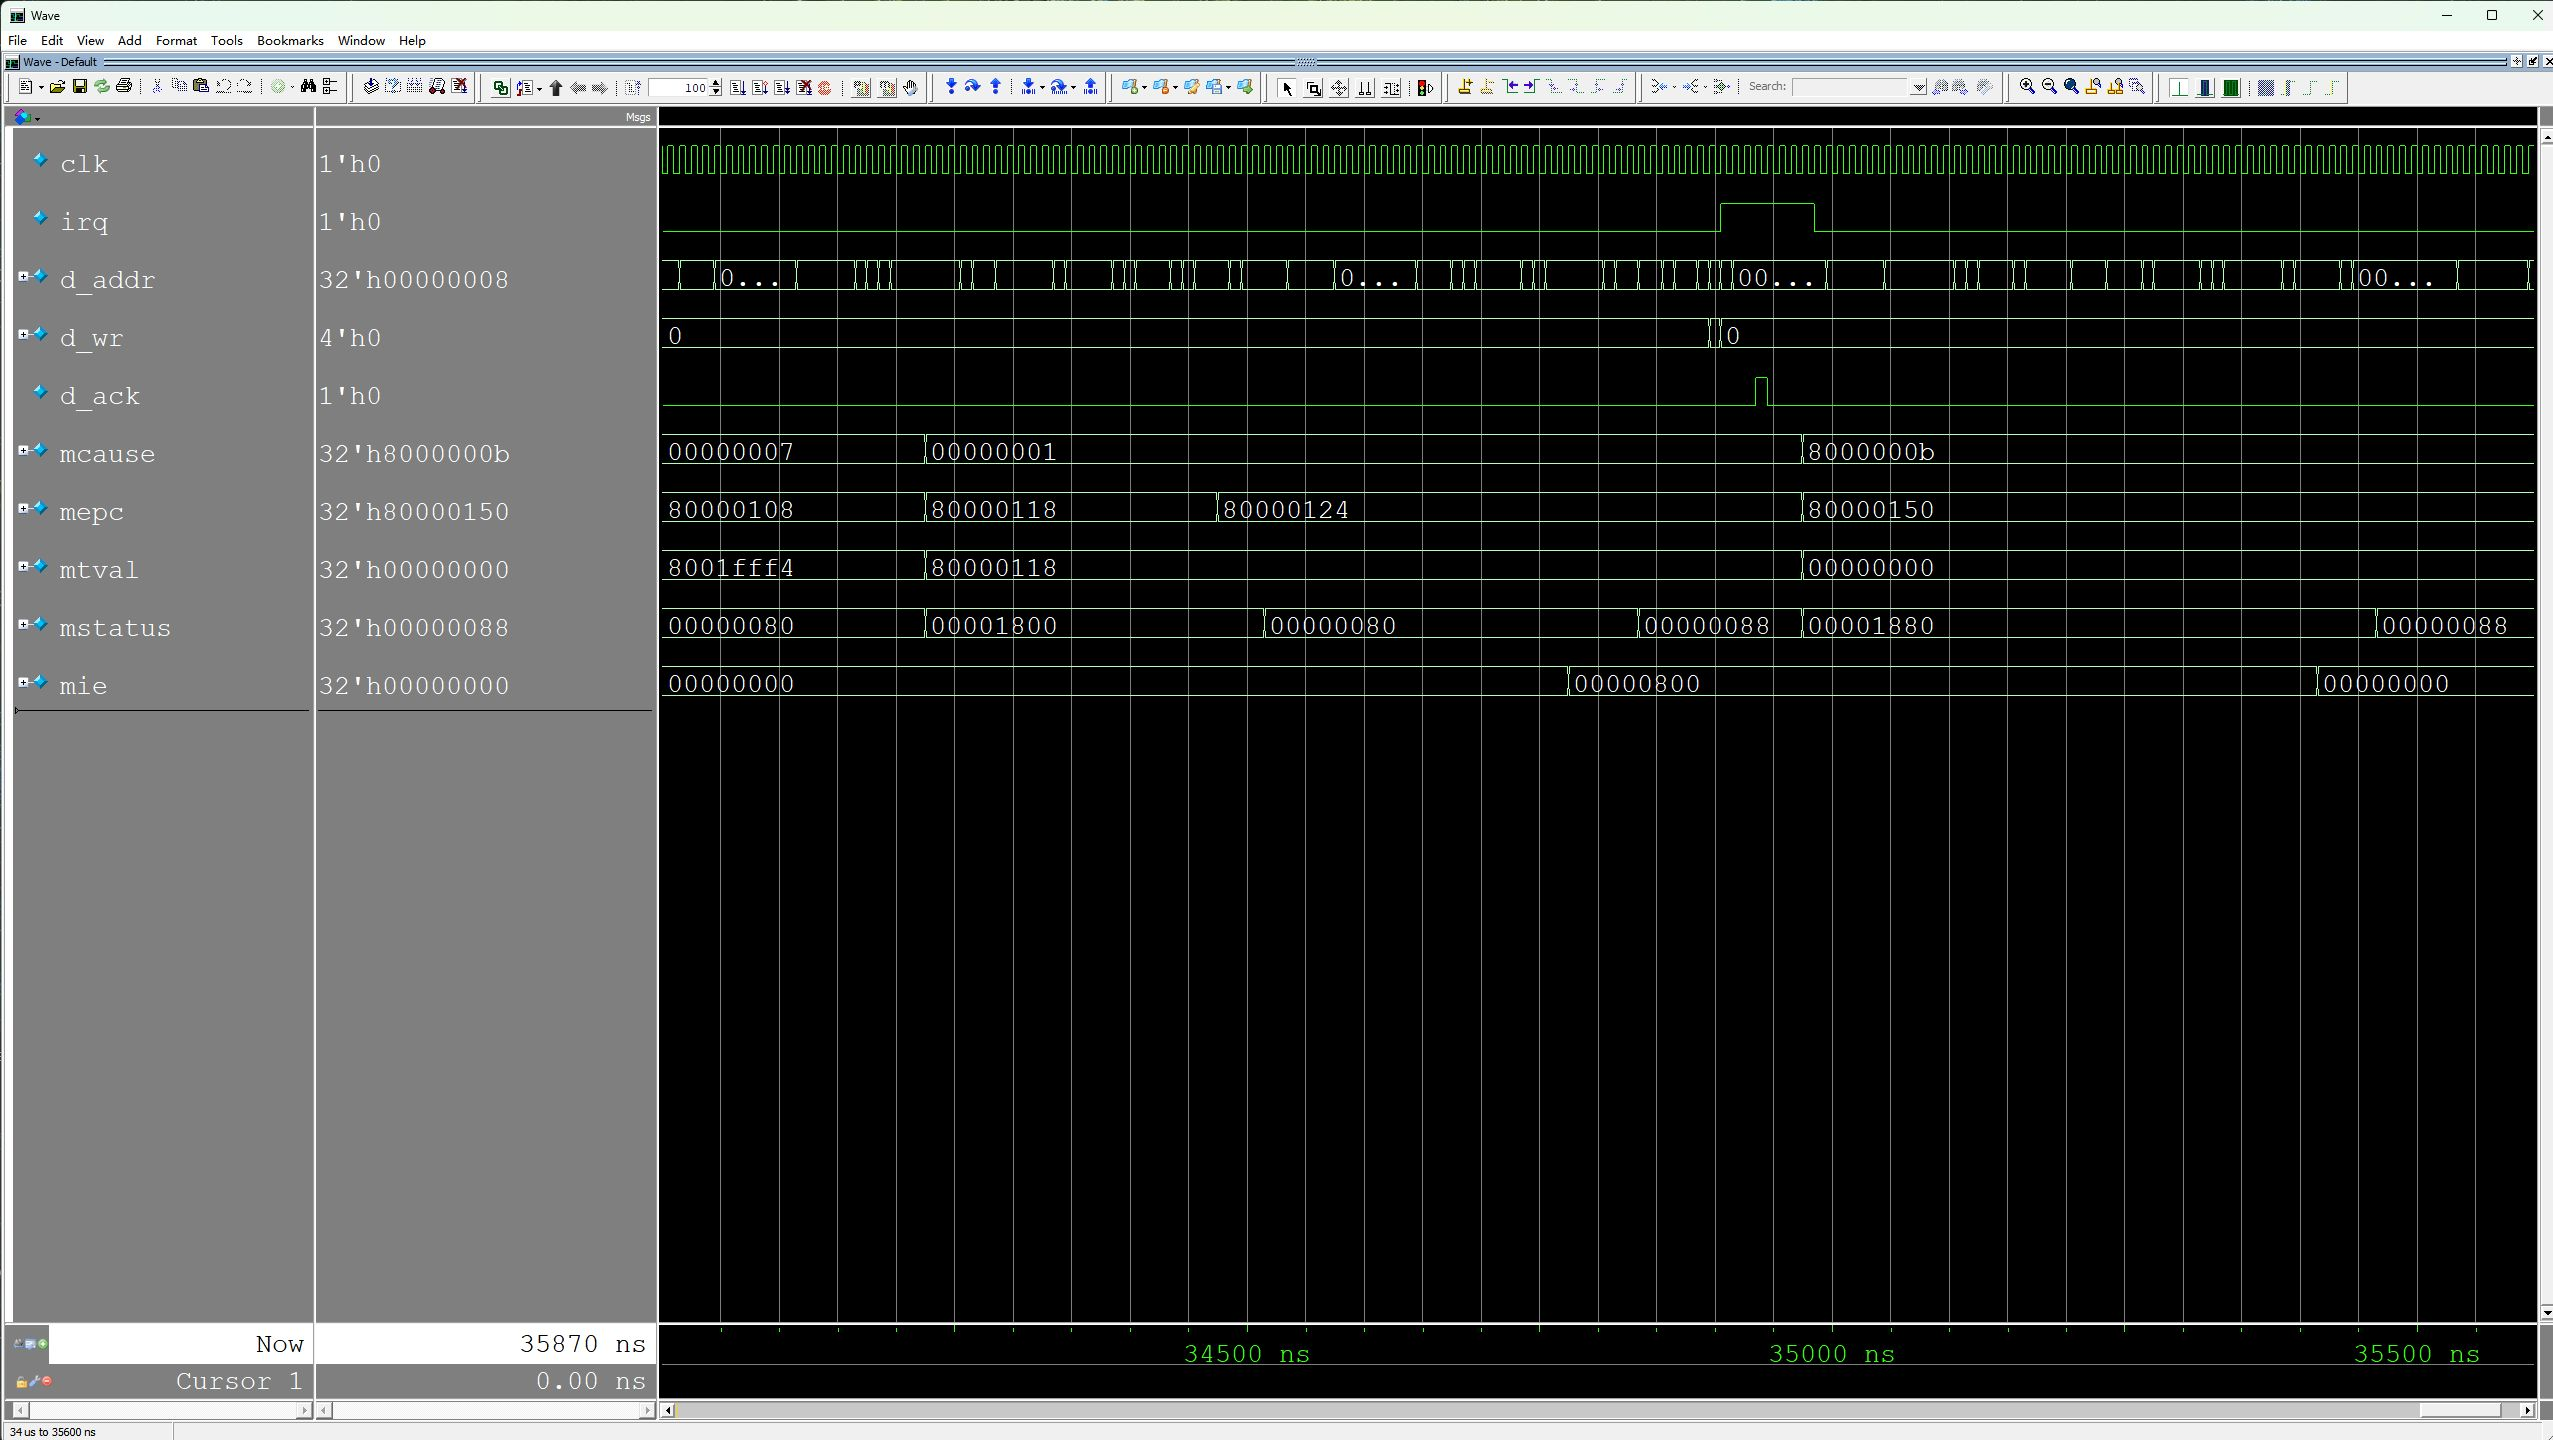
\includegraphics[width=0.8\linewidth]{../figure/cpu-system-external-irq-modelsim-original.jpg}
\caption{单发射整核的机器外部中断进入、CSR保存和MRET返回波形}
\label{fig:cpu-system-external-irq}
\end{figure}

\subsubsection{Cache访存与中断交互}

整核测试开启16\,KiB指令Cache和16\,KiB数据Cache，两者均为两路组相联、32\,B缓存行，数据Cache采用写回与写分配。
启动程序从片上SRAM复制测试代码到私有可缓存区，执行\texttt{FENCE.I}后转入该区；测试程序与中断处理程序均通过指令Cache取指。
测试台在数据Cache命中返回、缺失填充等待和缺失加载返回三个时刻分别驱动外部中断，结果见表\ref{tbl:cpu-cache-irq}。

\begin{reporttable}
\begin{longtable}{@{}p{0.19\linewidth}p{0.36\linewidth}p{0.24\linewidth}p{0.10\linewidth}@{}}
\caption{Cache开启时的外部中断场景}\label{tbl:cpu-cache-irq}\\
\toprule
场景 & 中断触发条件 & 保存的\texttt{mepc} & 结果 \\
\midrule
\endfirsthead
\caption[]{Cache开启时的外部中断场景（续）}\\
\toprule
场景 & 中断触发条件 & 保存的\texttt{mepc} & 结果 \\
\midrule
\endhead
\bottomrule
\endfoot
命中返回 & 驻留数据加载返回，不产生新的下层填充 & \texttt{0x80004060} & PASS \\
填充等待 & 缺失读事务已接纳，下层尚未返回数据 & \texttt{0x80004094} & PASS \\
缺失返回 & 新缓存行填充完成，目标加载返回 & \texttt{0x800040C8} & PASS \\
\end{longtable}
\end{reporttable}

三次中断入口均检查\texttt{mcause}=\texttt{0x8000000B}、\texttt{mtval}=0、\texttt{mstatus}=\texttt{0x1880}和\texttt{mie}=\texttt{0x800}。
处理程序清除\texttt{mie}，保持原\texttt{mepc}并执行\texttt{MRET}；返回后\texttt{mstatus}恢复为\texttt{0x88}，首条退休指令的PC等于原\texttt{mepc}。
三个目标加载分别得到\texttt{0x13579BDF}、\texttt{0x2468ACE0}和\texttt{0x31415926}，各加载及其后继指令均只退休一次，软件计数依次为1、2、3。

图\ref{fig:cpu-system-cache-irq}展示填充等待场景：\texttt{irq}在114590\,ns置位，随后下层返回缓存行并完成加载，115395\,ns进入中断，115855\,ns执行\texttt{MRET}。
外部中断有效且读事务待完成、下层无有效返回的状态累计持续66周期。
整次自检完成11758周期、1110次退休和12655项检查，包含三次中断进入、三次返回及三次恢复执行。
将处理程序中的\texttt{mepc}故意加4后，返回地址检查检出错误，测试入口返回1。

\begin{figure}[!htbp]
\centering
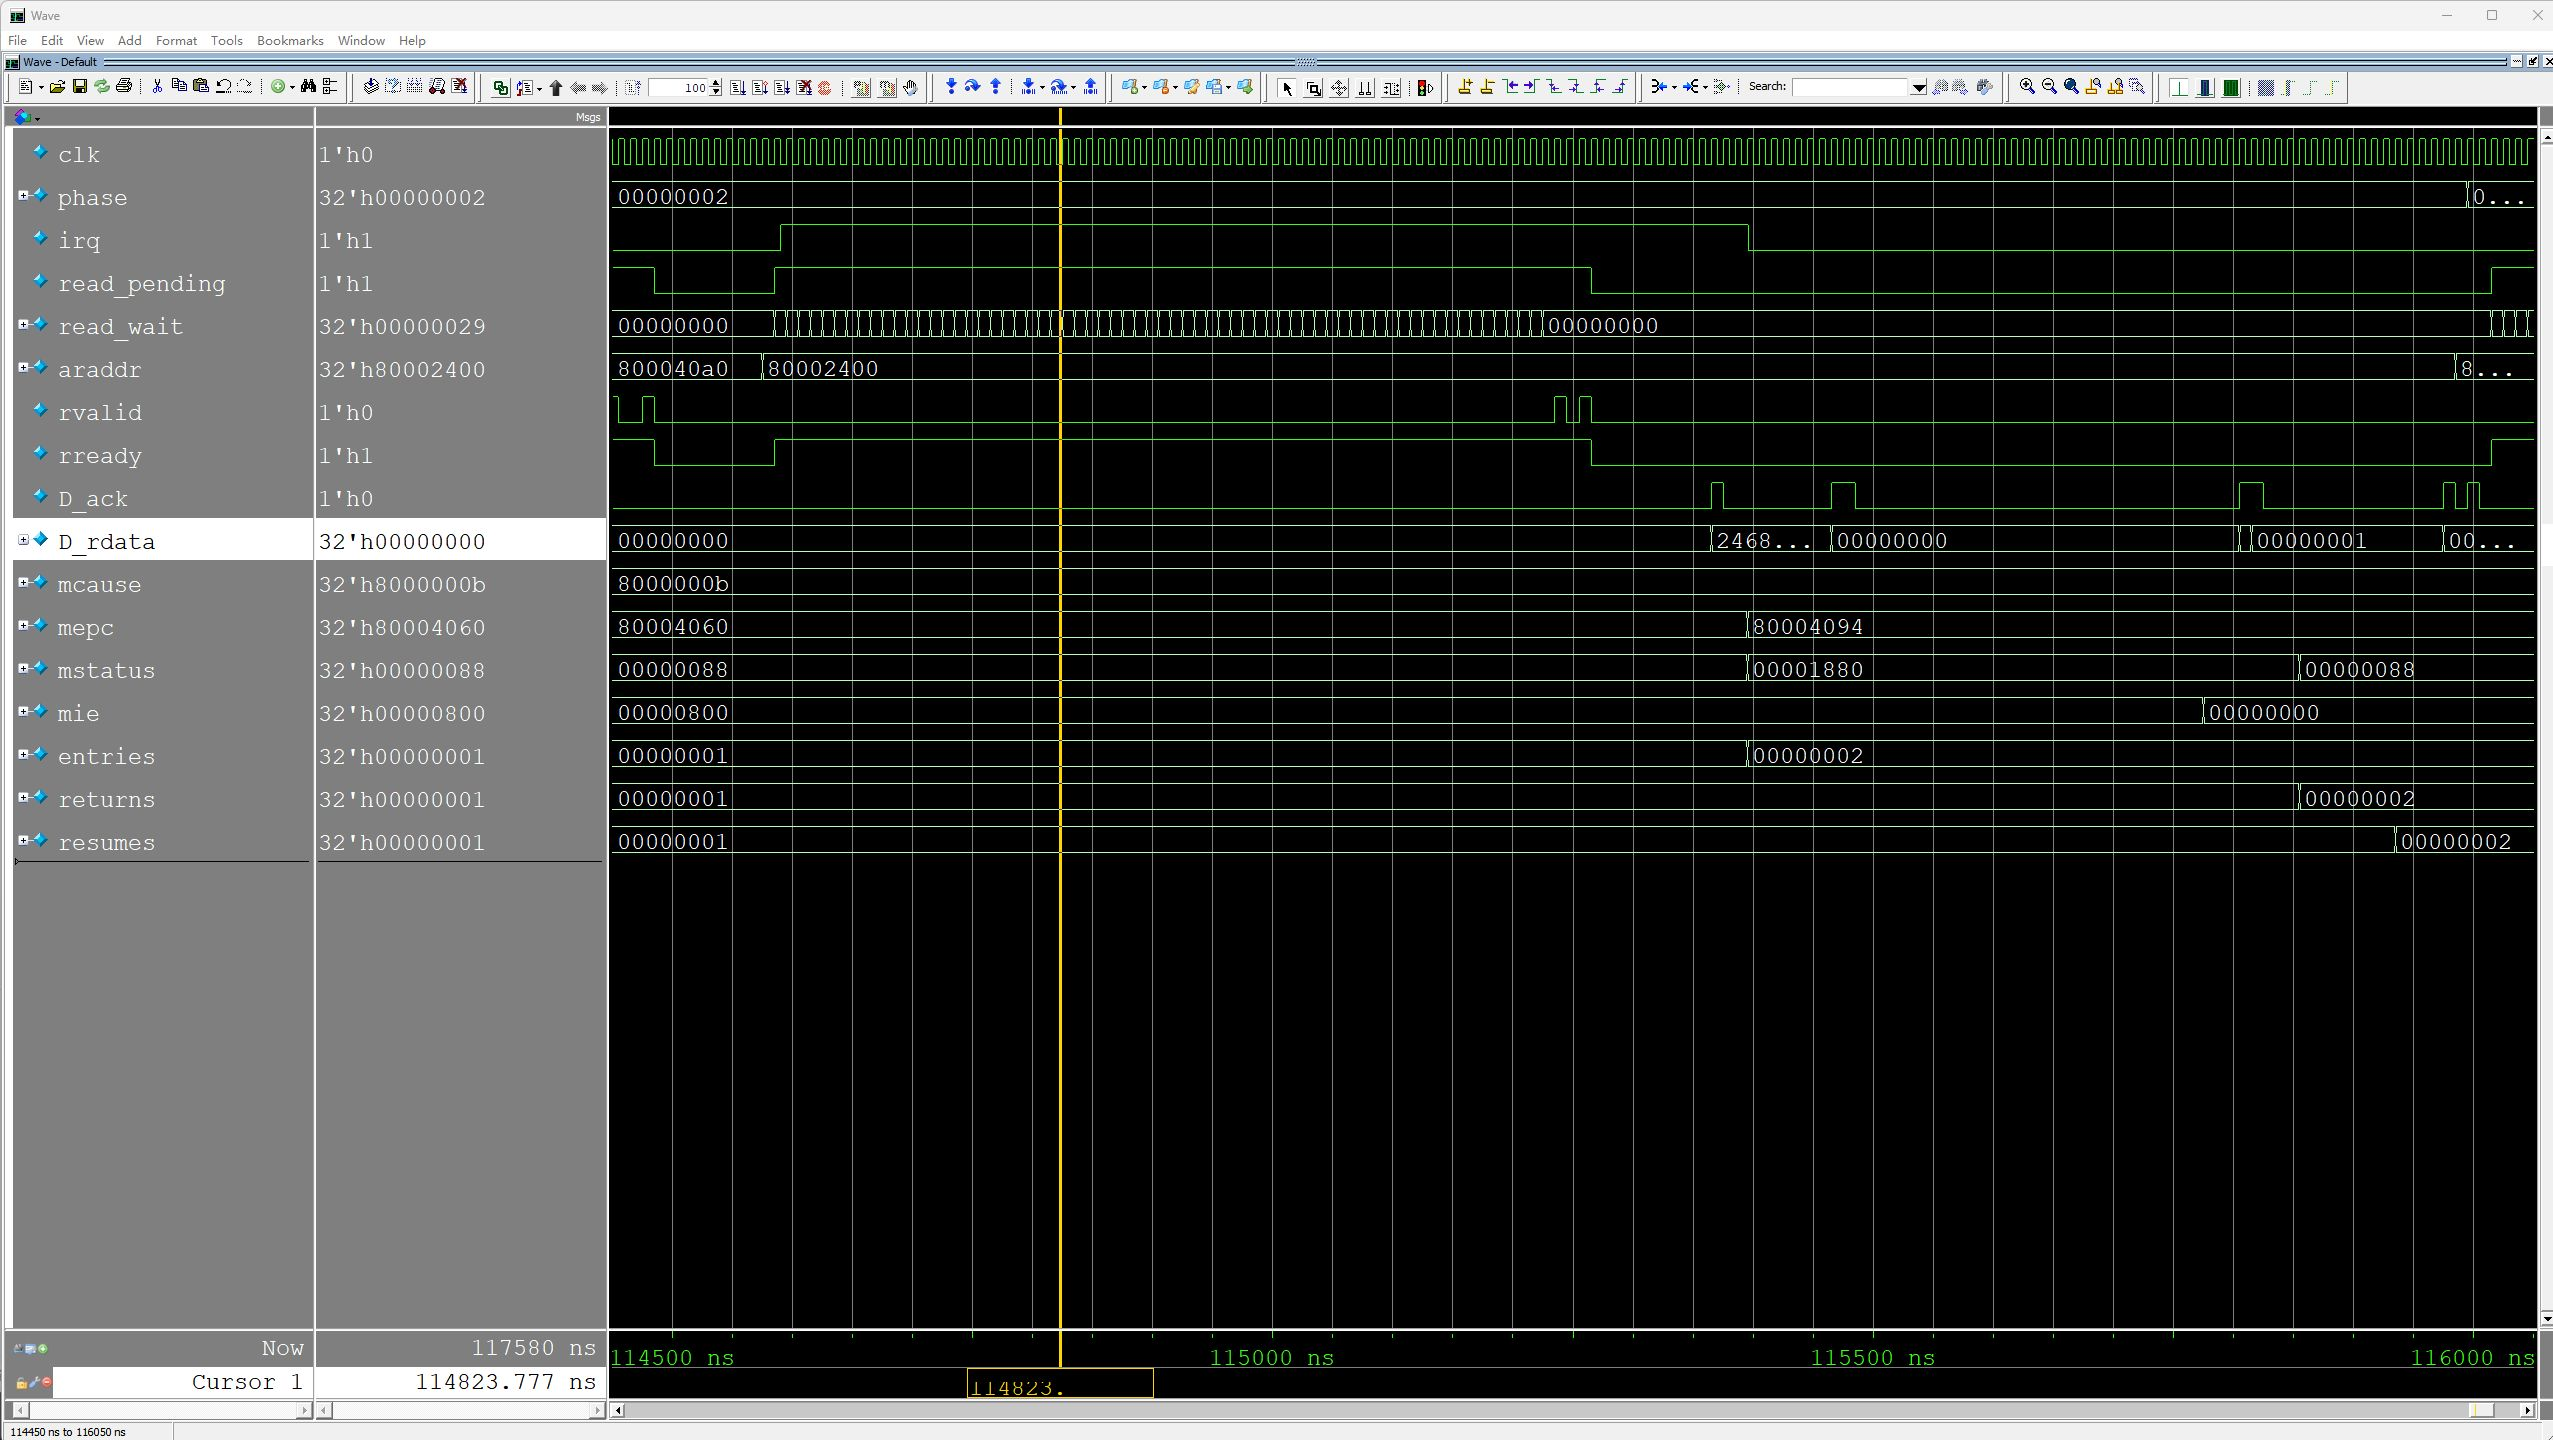
\includegraphics[width=0.8\linewidth]{../figure/cpu-system-cache-irq-modelsim-original.jpg}
\caption{Cache缺失填充等待期间的中断请求、加载完成与MRET返回波形}
\label{fig:cpu-system-cache-irq}
\end{figure}

\subsubsection{流水冲刷后的副作用隔离}

整核测试通过公开取指和数据端口运行定向固件，分别检查分支误预测重定向与加载访问异常后的后续指令。
三处分支的错误路径分别放置SRAM存储、MMIO写入和\texttt{mscratch}写入；四处长延迟错误加载后分别放置这三类写入及一条写同一目的寄存器的加载。
测试台在请求接纳前插入背压，将加载返回延迟设为32或64周期，并以\texttt{0xDEAFBEEF}作为错误响应和无效响应周期的数据。
表\ref{tbl:cpu-squash-cases}列出七个检查场景。

\begin{reporttable}
\begin{longtable}{@{}p{0.23\linewidth}p{0.22\linewidth}p{0.38\linewidth}p{0.08\linewidth}@{}}
\caption{流水冲刷后的副作用隔离测试}\label{tbl:cpu-squash-cases}\\
\toprule
触发条件 & 后续指令 & 检查结果 & 状态 \\
\midrule
\endfirsthead
\caption[]{流水冲刷后的副作用隔离测试（续）}\\
\toprule
触发条件 & 后续指令 & 检查结果 & 状态 \\
\midrule
\endhead
\bottomrule
\endfoot
分支误预测重定向 & SRAM存储 & 受保护字保持\texttt{0x13579BDF} & PASS \\
分支误预测重定向 & MMIO写入 & 仅有一次合法的\texttt{0x42}写入 & PASS \\
分支误预测重定向 & CSR写入 & \texttt{mscratch}保持\texttt{0x12345678} & PASS \\
加载访问异常 & SRAM存储 & 无额外存储，受保护字不变 & PASS \\
加载访问异常 & MMIO写入 & 无额外外设写入 & PASS \\
加载访问异常 & CSR写入 & 无额外CSR写入 & PASS \\
加载访问异常 & 同目的寄存器加载 & 后续请求未接纳；返回后重新加载正确值 & PASS \\
\end{longtable}
\end{reporttable}

七条禁止执行的指令均被取回，退休流中均未出现；其中四条异常后的后续指令进入译码。
四次异常均保存故障加载的PC，\texttt{mcause}=5、\texttt{mtval}=\texttt{0x8001F080}，故障加载不改变目的寄存器。
处理程序跳过故障片段后执行\texttt{MRET}，随后四次加载复用同一目的寄存器\texttt{x20}，均返回\texttt{0x11223344}。
两组返回延迟分别完成750周期、2199项检查和1102周期、3031项检查，各退休162条指令，完整退休序列一致。
另设四组错误输入：分别反转三处分支条件及将加载错误响应改报成功，均触发副作用检查失败。

图\ref{fig:cpu-system-squash}展示第一次加载访问异常：2285\,ns返回错误响应，随后产生\texttt{squash}并转入异常入口；\texttt{mepc}保存\texttt{0x800000C0}、\texttt{mcause}置为5，\texttt{mscratch}始终保持原值。
异常返回后，恢复加载使\texttt{recovered}由0变为1。
该场景验证阻塞式LSU等待期间禁止接纳后续请求，以及异常后的恢复执行。
本组测试不实例化Cache，MMIO由测试台状态模型提供；冻结输入、原始波形、退休流和运行索引见\path{docs/verification/cpu/system_support/SQUASH_README.md}。

\begin{figure}[!htbp]
\centering
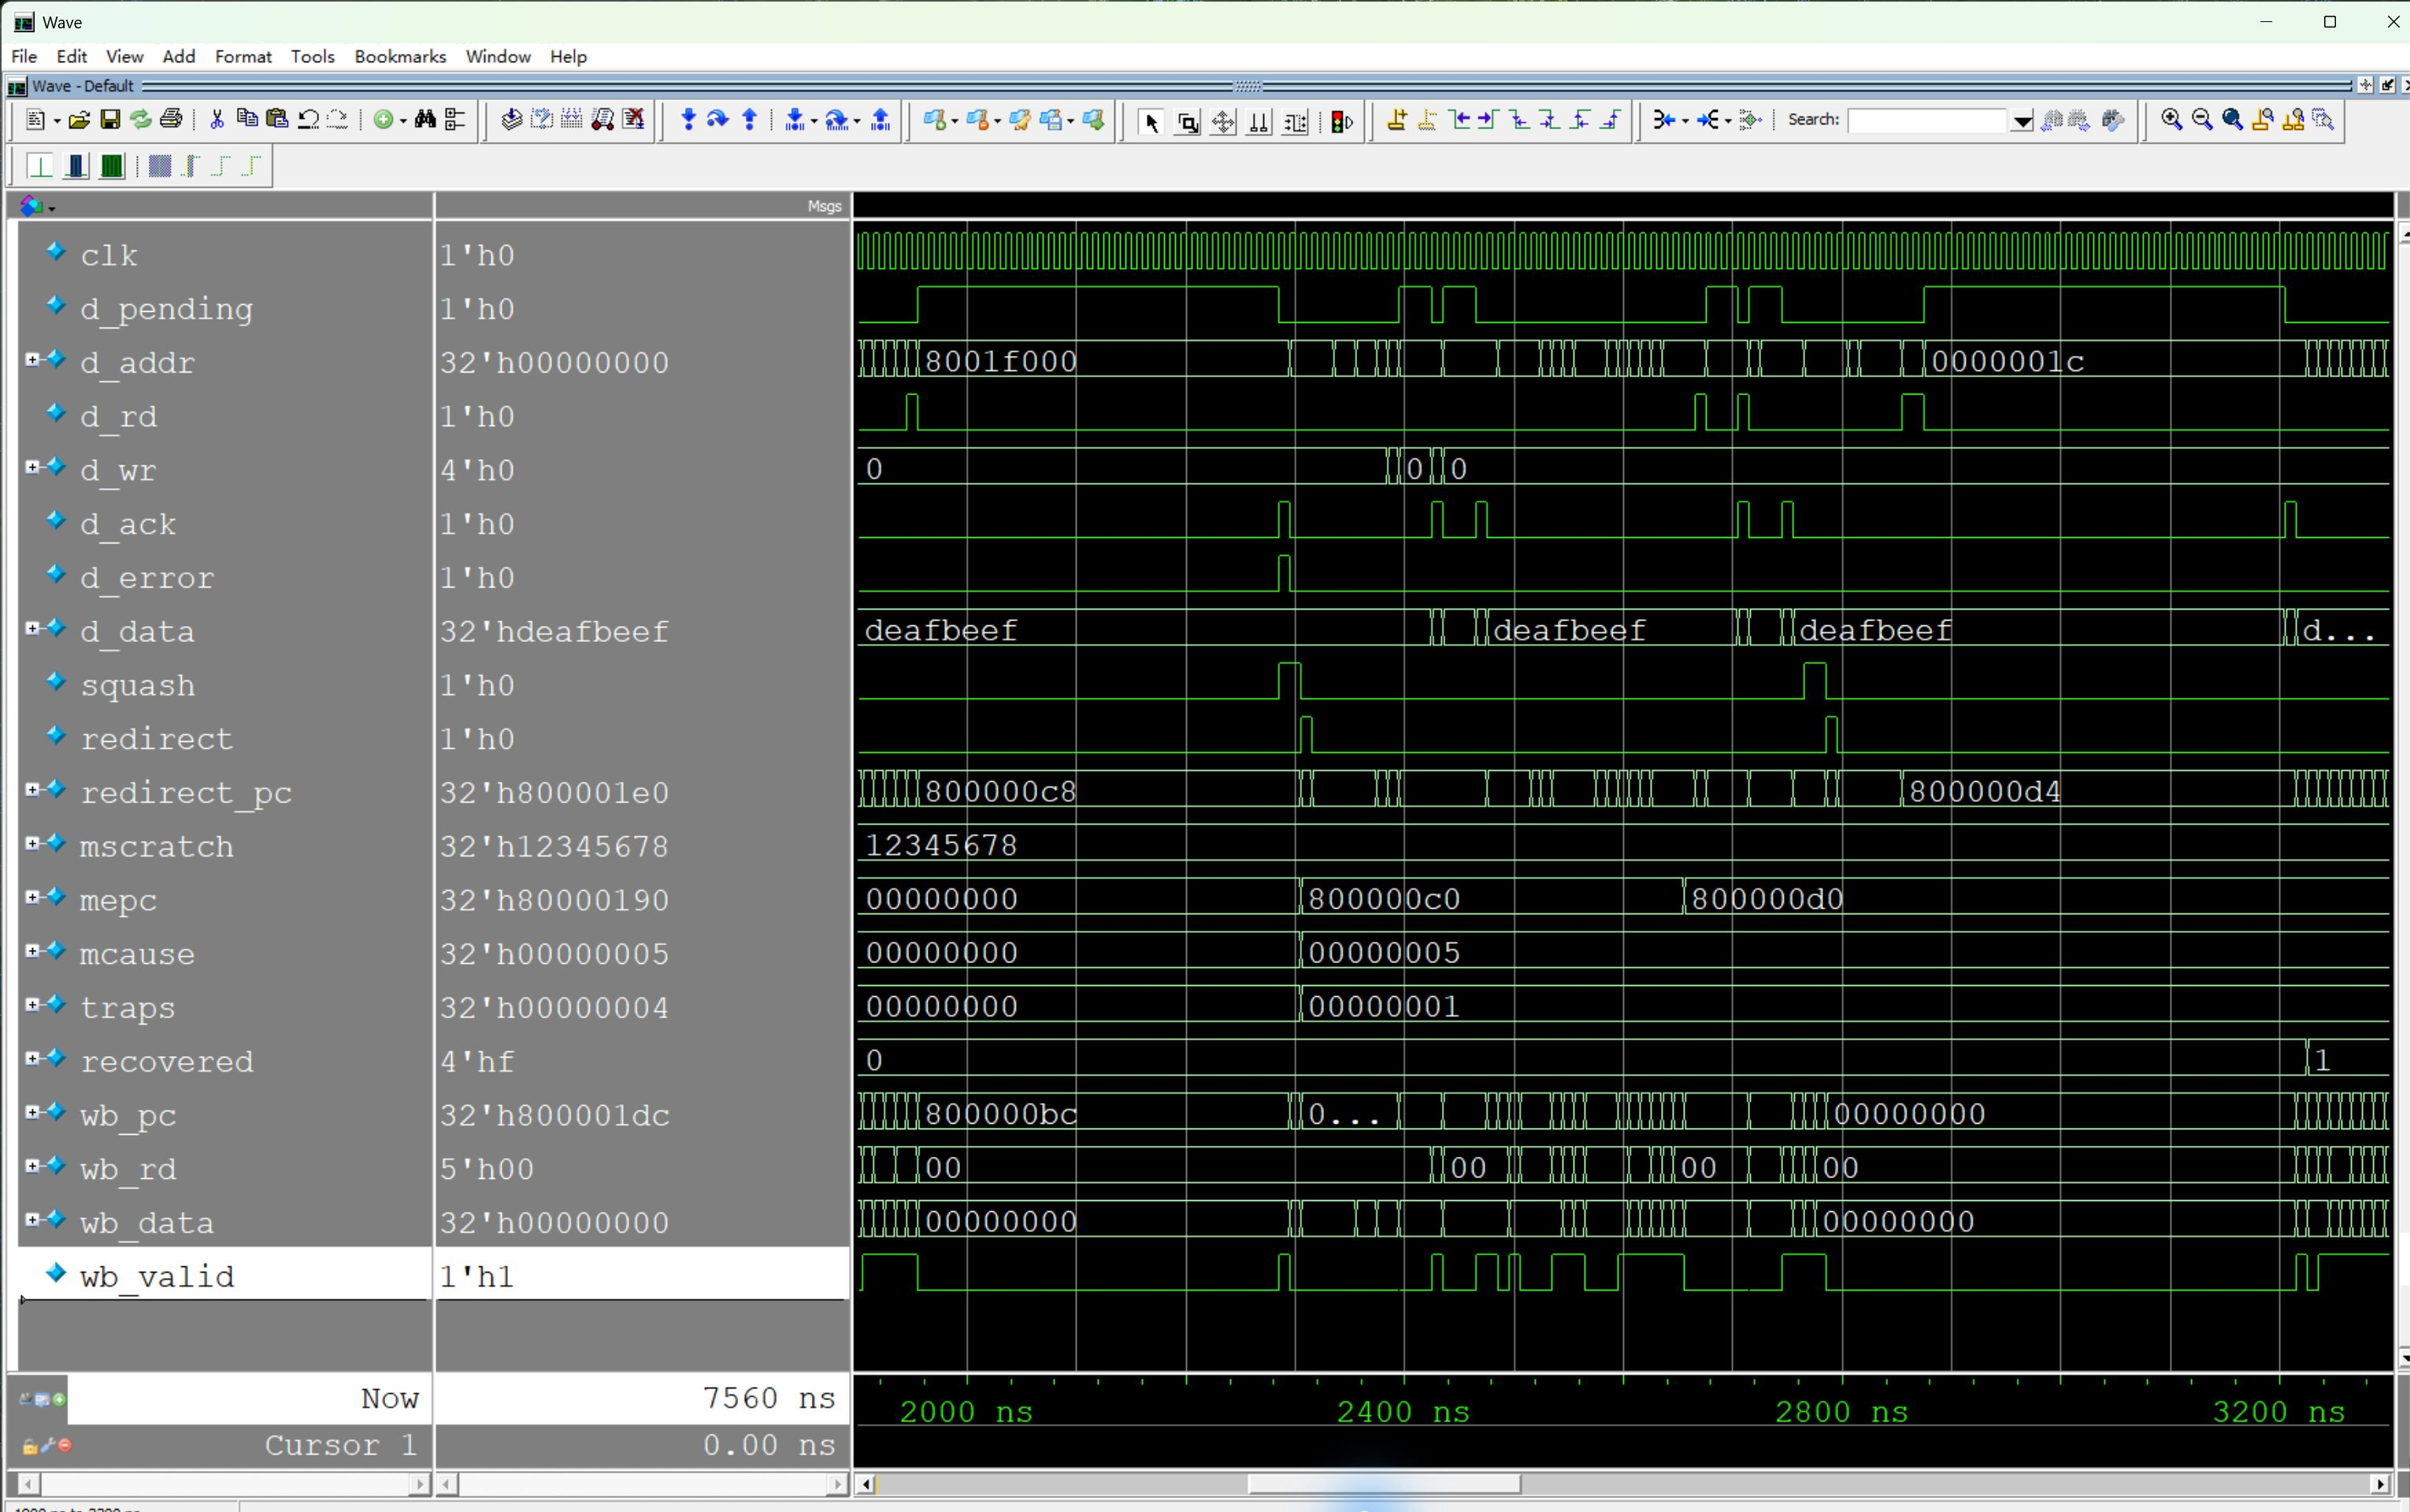
\includegraphics[width=0.8\linewidth]{../figure/cpu-system-squash-modelsim-original.jpg}
\caption{长延迟加载错误、流水冲刷和异常返回后的恢复加载波形}
\label{fig:cpu-system-squash}
\end{figure}


\subsubsection{发射宽度与Cache配置组合}

\texttt{DUAL\_ISSUE}与\texttt{CACHE\_ENABLE}分别选择单/双发射和I/D Cache开关。
ModelSim在CPU与存储子系统测试、SoC运行时测试中各覆盖四种组合，八组测试均通过。
表\ref{tbl:cpu-config-matrix}列出各次运行的双指令配对周期及B通路WB事件，两个数值均为完整测试运行的观测计数。
单发射组合的配对周期和B通路WB事件均为零，双发射组合均观测到第二通路实际工作。

\begin{reporttable}
\begin{longtable}{@{}p{0.18\linewidth}p{0.16\linewidth}p{0.28\linewidth}p{0.28\linewidth}@{}}
\caption{发射宽度与Cache配置组合验证}\label{tbl:cpu-config-matrix}\\
\toprule
发射配置 & Cache & CPU测试：配对/WB1 & SoC测试：配对/WB1 \\
\midrule
\endfirsthead
\caption[]{发射宽度与Cache配置组合验证（续）}\\
\toprule
发射配置 & Cache & CPU测试：配对/WB1 & SoC测试：配对/WB1 \\
\midrule
\endhead
\bottomrule
\endfoot
单发射 & 开启 & 0 / 0 & 0 / 0 \\
单发射 & 关闭 & 0 / 0 & 0 / 0 \\
双发射 & 开启 & 39 / 34 & 80 / 72 \\
双发射 & 关闭 & 25 / 22 & 80 / 72 \\
\end{longtable}
\end{reporttable}

PDS综合与器件映射另检查单发射＋Cache开启、双发射＋Cache关闭及双发射＋Cache开启三种组合，实际展开参数与目标配置一致。
该映射检查用于核对参数传递及生成结构，板级时序采用第三部分列出的独立后布线结果。
记录归档于\path{docs/verification/cpu/report_configurable_issue_2026-11-02/}中的参数矩阵文件；指令集回归和定向接口仿真按各自配置统计。

\subsubsection{双发射关键接口定向验证}

本组仿真针对双发射配置的队列出队、整数结果寄存、分支恢复、乘法早期旁路及LSU元数据接口，使用ModelSim执行定向测试。
输入清单、源码校验值、逐周期观测和原始日志登记于\path{docs/verification/cpu/diagram_review2_2026-11-02/}。
该双发射配置的定向检查结果见表\ref{tbl:dual-contract-tests}。

\begin{reporttable}
\begin{longtable}{@{}p{0.21\linewidth}p{0.58\linewidth}p{0.12\linewidth}@{}}
\caption{双发射关键接口定向检查}\label{tbl:dual-contract-tests}\\
\toprule
检查对象 & 覆盖与观测结果 & 状态 \\
\midrule
\endfirsthead
\caption[]{双发射关键接口定向检查（续）}\\
\toprule
检查对象 & 覆盖与观测结果 & 状态 \\
\midrule
\endhead
\bottomrule
\endfoot
FIFO组件 & 20821步，包含写指针2008次回绕与读指针1926次回绕；组件允许的操作与CPU出队约束分别检查 & PASS \\
整核分支与双槽 & 156周期、9个保持周期、4次恢复、3次陷入，包含错误路径Store抑制、B槽ALU取消、前序加载保持及恢复交叠 & PASS \\
CPU出队及ALU寄存 & 在上述整核程序中逐周期检查B出队必须伴随A出队；非保持沿后两路结果等于沿前组合ALU结果 & PASS \\
乘法早期元数据 & 41027个样本，对照完整写回值与早期值及其可用条件 & PASS \\
取指重定向 & 4次重定向，输出12包、丢弃4包；检查错误路径返回不进入恢复指令流 & PASS \\
LSU元数据FIFO & 深度2与深度4各10001周期，检查组件空、满及同时出入队行为 & PASS \\
\end{longtable}
\end{reporttable}

原强制输入零比较配对测试出现期望B发射而实际未发射，失败定位于夹具未同步提供简单ALU资格、寄存器角色、操作数零标志及预测下一PC，且配对预期沿用了旧策略。
完整驱动现行接口的后继夹具通过6168个检查点；原测试、断言和FAIL记录保留，未修改发射RTL。

真实取指、预译码、FIFO、发射及LSU路径的72次定向程序结果见表\ref{tbl:cpu-zero-pair-program}。
零比较用例按BEQ/BNE、\texttt{x0}位于rs1/rs2、B为ALU/Load/Store组合；每次程序还检查A生成数据、B等待后存储的RAW序列。
确认不跳转时允许后继访存，未确认或跳转时禁止后续LSU请求；推测ALU在恢复或异常时取消，并按PC检查写回值及外部访存次数。

\begin{reporttable}
\begin{longtable}{@{}p{0.31\linewidth}p{0.49\linewidth}p{0.12\linewidth}@{}}
\caption{双发射零比较分支与恢复的整核定向验证}\label{tbl:cpu-zero-pair-program}\\
\toprule
场景 & 主要观测 & 结果 \\
\midrule
\endfirsthead
\caption[]{双发射零比较分支与恢复的整核定向验证（续）}\\
\toprule
场景 & 主要观测 & 结果 \\
\midrule
\endhead
\bottomrule
\endfoot
操作数就绪且确认不跳转 & 12次目标配对；ALU、Load和Store正常完成 & 12/12 PASS \\
实际跳转、冷启动预测未命中 & 12次恢复，4个推测ALU取消，8个LSU后继无外部请求或退休 & 12/12 PASS \\
前序Load至A分支RAW & 累计等待108拍，12次取得加载前递后配对，B不越过A & 12/12 PASS \\
分支目标不对齐异常 & 12次陷入与MRET；4个推测ALU取消，LSU后继不执行 & 12/12 PASS \\
前序Load至B的RAW & 12次B阻塞，A先发射，B取得结果后独立执行 & 12/12 PASS \\
普通双源分支对照 & 6种组合各重复两次；4个简单ALU配对，8个LSU后继独立执行 & 12/12 PASS \\
\end{longtable}
\end{reporttable}

当前FIFO队首出队约束下的前递检查另通过694800个检查点，覆盖两路数据与零标志、六级前递优先级、RF写入、复位及X/Z。
保留失败包括3次旧夹具运行和9次诊断/故障注入；错误开放LSU配对、禁止B取消及破坏零标志均触发相应断言。
源码版本标识、逐拍记录、覆盖矩阵和完整通过/失败记录见\path{docs/verification/cpu/document_review_zero_pair_20261102/}。
本组结果对应上述配置下的零比较分支配对与前递定向仿真。

